\documentclass[a4paper,twocolumn,11pt]{article}

\usepackage[utf8]{inputenc}
\usepackage[T1]{fontenc}
\usepackage{amsmath,amssymb,amsfonts}
\usepackage{graphicx}
\usepackage{hyperref}
\usepackage{booktabs}
\usepackage{xcolor}
\usepackage{enumitem}
\usepackage{float}
\usepackage{geometry}
\geometry{margin=20mm}

\graphicspath{{../figures/}}

\hypersetup{
  colorlinks=true,
  linkcolor=blue!60!black,
  citecolor=blue!60!black,
  urlcolor=blue!60!black,
  hypertexnames=false
}

\title{Counter-Evidence of Diff\'erance:\\A Refutation from Engineering and Mathematics}

\author{Yuichiro Nishi\\{\small \texttt{yuichiro@yuichironishi.com}}\\{\small ORCID: \href{https://orcid.org/0009-0006-3823-0313}{0009-0006-3823-0313}}}

\date{\today}

\begin{document}

\maketitle

\begin{abstract}
Derrida's \emph{diff\'erance} claims that signification is always produced through differences and perpetually deferred---that meaning never reaches a determinate, present state. The claim is universal, constitutive, and admits no domain in which signification is exempt. This paper tests that universal claim against engineering and mathematics.

The test fails for the universal claim.

In Transformer architecture, the attention mechanism computes relevance through inner products of embedding vectors: an operation undefined unless both operands are determinate numerical vectors. At every forward pass, the softmax function yields a determinate probability distribution over the vocabulary, summing to exactly one. The signifying process reaches bounded computational closure: the same input produces the same output, generation halts on its own, and model weights do not drift during inference. These are not claims about semantic presence; they are claims about operational determinacy. Universal \emph{diff\'erance}---as a thesis about signification in general---is incompatible with operational determinacy of this strength.

The Transformer evidence is measurement: reproducible across three independently trained Transformer families (GPT-2, Pythia, TinyLlama), verified by scripts that any researcher can execute, covering 26 properties (eight per model and two across models).

The refutation is not limited to Transformers, nor does it rest on measurement alone. Shannon's channel coding theorem is a \emph{theorem}: it guarantees signifier recovery through noisy channels at rates below capacity, and recovery succeeds billions of times per second under that guarantee. Formally verified compilation (CompCert) is a \emph{machine-checked proof}: it establishes meaning-preservation across sign-system transformations within the fragment where the formal guarantee holds. Mathematical structures such as $\pi$ and the imaginary unit are \emph{structural facts}: they are approximated independently across textual systems that did not share resources---what is constructed is the sign, what is discovered is the constraint the sign is forced to track. Measurement, theorem, and structural fact are three distinct types of evidence, and none of them is interpretation open to debate.

\emph{Diff\'erance} is also internally self-undermining under its universal reading: self-referentially paradoxical, unfalsifiable, performatively contradictory in its mode of communication, and itself a metaphysical thesis---a metaphysics of deferral replacing the metaphysics of presence.

No prior work has tested \emph{diff\'erance} against operational systems. Existing critiques have been philosophical or hermeneutic. This paper presents the first constructive refutation grounded in reproducible engineering. Gunkel (2025) identified certain computational facts in large language models and assigned them a Derridean interpretation; even granting that interpretive move locally, the universal thesis does not follow, because the pipeline as a whole reaches bounded determinate closure rather than endless deferral.

The play of differences is real. Its universalization as endless, constitutive deferral of any determinate state is not.
\end{abstract}

% ====================================================================
% SECTION 1: INTRODUCTION
% ====================================================================

\section{Introduction}
\label{sec:introduction}

\subsection{Diff\'erance as a Universal Claim}
\label{sec:universal}

In 1968, Jacques Derrida introduced \emph{diff\'erance}---a neologism combining the French \emph{diff\'erer} (to differ and to defer)---as a name for the condition of possibility of all signification. The thesis, as articulated across \emph{De la grammatologie}~\cite{Derrida1967,Derrida1976}, \emph{La diff\'erance}~\cite{Derrida1968,Derrida1982margins}, and \emph{Positions}~\cite{Derrida1972,Derrida1981}, holds that meaning is never self-present in a sign but is always produced through a play of differences and perpetually deferred along an endless chain of signifiers. No sign carries a positive, self-contained content; meaning arises only from what a sign is not.

Crucially, Derrida did not restrict the domain of applicability of this thesis. \emph{Diff\'erance} was not presented as a claim about literary texts, nor about a particular class of signs, nor about human consciousness alone. It was advanced as a condition of signification \emph{in general}---as the structure underlying all meaning-making whatsoever. In the 1968 lecture \emph{La diff\'erance}~\cite{Derrida1968}, Derrida states that \emph{diff\'erance} ``governs nothing, reigns over nothing, and nowhere exercises any authority''~\cite[p.~22]{Derrida1982margins}, yet simultaneously insists that ``the movement of signification is possible only if'' each present element bears within it the trace of another~\cite[p.~13]{Derrida1982margins}---a formulation that explicitly encompasses the totality of signification without exception.

A claim that encompasses the totality of signification without exception is a universal claim. It may not have been intended as an empirical hypothesis in the natural-scientific sense, but its scope is unrestricted: it asserts something about \emph{all} meaning, \emph{all} signs, \emph{all} signification. This scope is not an interpretation imposed from outside; it is the consequence of Derrida's own refusal to delimit the domain of \emph{diff\'erance}.

An anticipated objection must be addressed here: that treating \emph{diff\'erance} as a universal claim is itself an interpretive imposition---that Derrida himself stated \emph{diff\'erance} is ``neither a word nor a concept''~\cite[p.~3]{Derrida1982margins}, and that subjecting it to domain-general scrutiny misapplies an analytic framework to something operating in a different register.

Before addressing this objection, a prior question must be posed: if \emph{diff\'erance} is neither a word nor a concept, and possesses ``neither existence nor essence''~\cite[p.~6]{Derrida1982margins}, then what is it? Derrida does not answer this question. Yet he \emph{described} \emph{diff\'erance} as the condition of possibility of signification, \emph{argued} for it across multiple works, \emph{taught} it in lectures, and \emph{deployed} it as a premise in disputes with other thinkers. Each of these operations---describing, arguing, teaching, deploying as a premise---is a knowledge operation performed through conceptual means. There is a fundamental tension between the ontological status Derrida assigned to \emph{diff\'erance} (not a concept, not a word, possessing neither existence nor essence) and the work he required it to perform (serving as the condition of possibility of all signification). If \emph{diff\'erance} is irreducible to knowledge, it cannot function as a premise, a condition, or an explanation of anything. If it does function as these things---and Derrida's own texts require it to---then it is, \emph{de facto}, a conceptual claim, regardless of the status its author assigned to it.

This tension deepens the objection rather than resolving it, and produces a trilemma, each horn of which is fatal to the defense of \emph{diff\'erance}:

If \emph{diff\'erance} is not a universal claim, then it has a restricted domain. In that case, there exist domains---engineering, mathematics, computation---to which it does not apply, and in which the signifying process can reach operational determinacy. The defender has conceded the central point of this paper.

If \emph{diff\'erance} is a universal claim, then it is subject to scrutiny from every domain, including engineering and mathematics. This is the premise under which the present paper proceeds.

If \emph{diff\'erance} is neither a thesis nor a concept and makes no claim at all, then it contributes nothing to knowledge and is unfalsifiable in principle. By Popper's criterion~\cite{Popper1934}, it says nothing. By any criterion, it cannot obstruct the findings presented here.

The texts themselves resolve this trilemma. \emph{De la grammatologie}~\cite{Derrida1967,Derrida1976} applies \emph{diff\'erance} to the sign in general. \emph{La diff\'erance}~\cite{Derrida1968,Derrida1982margins} presents it as the condition of possibility of signification as such. \emph{Positions}~\cite{Derrida1972,Derrida1981} extends the same unrestricted scope through a series of dialogues in which \emph{diff\'erance} is discussed as the underlying structure of signification. These are not restricted applications. To read them as such would require ignoring their explicit scope---an interpretive move far more aggressive than the one this paper makes.

A universal claim carries a specific logical consequence: it must hold in every domain to which it applies. If \emph{diff\'erance} is the condition of possibility of all signification, then it must hold for signification as it occurs in engineering, in mathematics, and in computation---not merely in literary interpretation or philosophical discourse.

\subsection{A Single Counter-Example Suffices}
\label{sec:counter-example}

The logical structure of the situation is straightforward. A universal claim of the form ``for all $x$ in domain $D$, property $P$ holds'' is refuted by a single instance of $x$ in $D$ for which $P$ does not hold. This is not a matter of philosophical convention but of elementary logic, recognized equally by Popper's falsificationism, by classical predicate logic, and by mathematical proof by counterexample.

If \emph{diff\'erance} asserts that the signifying process \emph{never} reaches a determinate state, then a single domain in which the signifying process \emph{does} reach such a state in bounded time---in which the play of differences converges to a determinate, reproducible output---constitutes a refutation of the universal claim. The refutation need not explain the totality of human meaning-making. It need not address every text Derrida ever wrote. It needs only to exhibit one domain in which the thesis fails.

This paper exhibits several such domains.

\subsubsection{A Note on the Term ``Meaning''}

The word ``meaning'' carries different senses in different traditions: computational meaning (the value of a function at a point), linguistic meaning (what a word communicates to a speaker), phenomenological meaning (the lived experience of understanding), and Derrida's specific sense of \emph{signification} (the relation between signifier and signified). This paper presents counter-evidence primarily at the computational and formal levels: the determinacy of embeddings, the closure of probability distributions, the convergence of optimization, the recoverability of transmitted signals.

This restriction does not weaken the refutation. \emph{Diff\'erance} claims to be the condition of possibility of signification \emph{in general}---it must hold at every level, including the computational. If it fails at the computational level, it fails as a universal claim. A universal claim does not require refutation at every level; it requires refutation at any one level. The counter-evidence need not address the phenomenology of human understanding to refute the universality of \emph{diff\'erance}.

\subsection{This Paper Presents Counter-Evidence, Not Critique}
\label{sec:not-critique}

A distinction must be drawn at the outset between critique and refutation, as these are fundamentally different operations.

Critique operates within the domain of interpretation and argumentation. It proposes that a thesis is internally inconsistent, poorly reasoned, or based on questionable premises. Critique can always be met with counter-critique; it initiates a dialogue within a shared discursive space. The history of responses to \emph{diff\'erance}---from Searle~\cite{Searle1977} to Habermas~\cite{Habermas1985} to Evink~\cite{Evink2020}---is a history of critique. These are arguments about arguments.

Refutation by counter-evidence operates differently. It does not argue that the thesis is poorly reasoned; it demonstrates that the thesis is contradicted by observable fact. The distinction is the same as that between arguing that a physical theory has internal problems and exhibiting an experimental result that the theory cannot accommodate. The former is a contribution to theoretical debate.

The latter is a termination condition.

This paper presents counter-evidence. It does not propose an alternative reading of Derrida, nor does it claim that Derrida's arguments are poorly constructed. It demonstrates that operational systems---systems whose behavior is observable, measurable, and reproducible---exhibit properties that are incompatible with \emph{diff\'erance} as a universal thesis. The counter-evidence consists of engineering facts, mathematical theorems, and computational operations whose outcomes can be independently verified by any reader with access to the relevant systems.

The refutation is constructive: it does not merely assert that \emph{diff\'erance} fails, but shows \emph{how} and \emph{where} it fails, at each stage of a precisely characterized computational pipeline, and through independent lines of evidence from communication theory, type theory, and mathematical physics.

\subsection{Prior Work and the Gap}
\label{sec:prior-work}

\subsubsection{Existing Critiques of Diff\'erance}

\emph{Diff\'erance} has been subject to sustained philosophical critique from multiple traditions over five decades. These critiques can be organized by method:

\textbf{Speech act theory.} Searle~\cite{Searle1977} argued that Derrida's reading of Austin misidentifies the role of intention in fixing meaning, and that iterability---the repeatability of signs across contexts---applies equally to speech and writing, collapsing the binary that Derrida sought to deconstruct.

\textbf{Performative contradiction.} Habermas~\cite{Habermas1985} charged that any critique of reason that employs reason's own tools while claiming to stand outside reason is self-undermining. The act of asserting that all meaning is unstable presupposes the stability of meaning sufficient to communicate the assertion.

\textbf{Formal logic.} Priest~\cite{Priest2002} translated \emph{diff\'erance} into the vocabulary of paraconsistent logic and diagonalization, identifying it as an instance of the Inclosure contradiction. Livingston~\cite{Livingston2010} attempted a systematic formalization of \emph{diff\'erance} through metalogic. Dutilh Novaes~\cite{DutilhNovaes2012} identified a critical scope mismatch: G\"odel incompleteness---the formal result most frequently analogized to \emph{diff\'erance}---is provably restricted to formal systems satisfying specific expressibility conditions, whereas \emph{diff\'erance} claims universal applicability.

\textbf{Internal philosophical critique.} Evink~\cite{Evink2020} argued that the temporization dimension of \emph{diff\'erance} retains a covert ``metaphysical desire for purity,'' rendering deconstruction itself thoroughly metaphysical. Sweetman~\cite{Sweetman1999} identified self-contradiction in the claim that all meaning is deferred. Ellis~\cite{Ellis1989} argued that deconstruction's ``alternative logic'' substitutes rhetorical devices for rigorous logical analysis.

\textbf{Science Wars.} Gross and Levitt~\cite{GrossLevitt1994} and Sokal and Bricmont~\cite{SokalBricmont1998} challenged postmodernist misappropriation of scientific concepts. Notably, Sokal and Bricmont explicitly declined to devote a chapter to Derrida, on the grounds that Derrida, unlike Lacan or Irigaray, does not systematically misuse scientific terminology.

\subsubsection{Adjacent Technical Work}

Several bodies of work approach the tension between information theory and \emph{diff\'erance} without directly confronting it. Dretske~\cite{Dretske1981} developed a naturalistic theory of meaning grounded in Shannon's information theory. Hayles~\cite{Hayles1999} argued that cybernetics introduces a pattern/randomness dialectic that supersedes Derrida's presence/absence dialectic. Lafontaine~\cite{Lafontaine2007} and Geoghegan~\cite{Geoghegan2023} demonstrated historically that French post-structuralism was substantially shaped by cybernetic and information-theoretic concepts.

Most recently, Gunkel~\cite{Gunkel2025} argued in ``The Diff\'erance Engine'' that large language models \emph{actualize} \emph{diff\'erance} computationally. This paper reaches the opposite conclusion from the same technical object, as we discuss in Sec.~\ref{sec:gunkel}.

\subsubsection{The Gap}

The existing literature reveals a clear gap. All critiques of \emph{diff\'erance} to date have been philosophical, logical, or hermeneutic---they operate at the level of interpretation and argumentation. No prior work has presented a constructive refutation grounded in reproducible engineering and formal systems.

This gap has a structural explanation. \emph{Diff\'erance} was formulated in terms that do not directly invoke scientific or mathematical concepts (as Sokal and Bricmont noted), making it resistant to the kind of terminological critique that proved effective against Lacan or Irigaray. The refutation must therefore take a different route: not exposing misuse of technical vocabulary, but testing the \emph{content} of the universal claim against systems whose operational behavior is observable and measurable.

This paper fills that gap.

Let it be stated again. This is not critique. It is refutation.


% ====================================================================
% SECTION 2: TRANSFORMER ARCHITECTURE
% ====================================================================

\section{Transformer Architecture and the Levels of Determination}
\label{sec:transformer}

\subsection{Overview: The Pipeline}
\label{sec:pipeline}

The Transformer is a computational architecture, introduced by Vaswani et al.~\cite{Vaswani2017}, that processes sequences of discrete symbols (tokens) and produces sequences of discrete symbols as output. It is the architecture underlying all contemporary large language models. When such a system receives a text prompt and generates a coherent response, it does so through a pipeline of deterministic mathematical operations. Each operation takes determinate numerical inputs and produces determinate numerical outputs.

The pipeline can be decomposed into five levels, each of which involves a distinct type of determination. Before describing the pipeline, Table~\ref{tab:terminology} maps the philosophical vocabulary of \emph{diff\'erance} to the engineering and mathematical concepts examined in this paper. Entries marked with $\rightarrow$ indicate claims of \emph{diff\'erance} for which no structural counterpart exists in the system.

\begin{table}[ht]
\centering
\caption{Each claim of \emph{diff\'erance} is tested at a specific operational layer of the Transformer pipeline. The right column names that layer. It is not a semantic identification of the philosophical concept with the computational object; it is the site at which the claim on the left is operationally confronted.\label{tab:terminology}}
\small
\begin{tabular}{@{}p{0.30\columnwidth}p{0.52\columnwidth}r@{}}
\toprule
Claim of \emph{Diff\'erance} & Operational Layer Where the Claim Is Tested & Sec. \\
\midrule
Signification & Determinate probability distribution over vocabulary & 2.5 \\
Play of differences & Attention weight computation & 2.3 \\
Presence & Determinate output at each forward pass (operational) & 2.5 \\
Deferral & $\rightarrow$ No corresponding layer: computation is simultaneous & 2.3 \\
Positive content of sign & Embedding vector with fixed numerical values & 2.2 \\
Endless chain of signifiers & $\rightarrow$ Terminated by EOS token & 2.6 \\
Indeterminacy & $\neq$ Stochasticity: the distribution itself is determinate & 3.2 \\
\bottomrule
\end{tabular}
\end{table}

Fig.~\ref{fig:pipeline} provides an overview of the pipeline; the remainder of this section examines each level in detail.

\begin{figure*}[t]
\centering
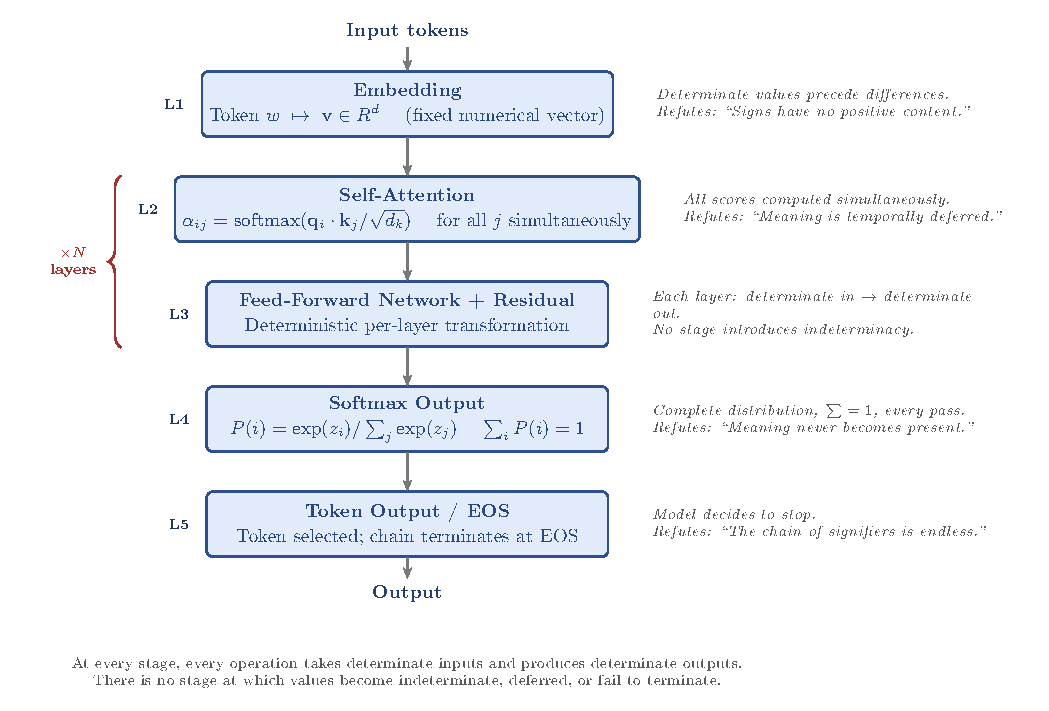
\includegraphics[width=\textwidth]{pipeline.pdf}
\caption{The Transformer pipeline. Each level involves a distinct type of determination, examined in Secs.~\ref{sec:embedding}--\ref{sec:irreversibility}. Right column shows the claim of \emph{diff\'erance} refuted at each stage.\label{fig:pipeline}}
\end{figure*}

There is no stage at which values become indeterminate, no stage at which determination is deferred, and no stage at which the computation fails to terminate.

\subsection{Level 1---Embedding: Determinate Values Precede Difference}
\label{sec:embedding}

For a Transformer to process language, each token must first be converted into a mathematical object that admits arithmetic operations. This conversion is called \emph{embedding}: each token is mapped to a point in a high-dimensional continuous space.

Concretely, each token $w$ in the vocabulary is assigned a vector of dimension $d$:
\begin{equation}
\mathbf{v} = (v_1, v_2, \ldots, v_d)
\end{equation}
In GPT-3, $d = 12{,}288$. Each component $v_i$ is a definite real number. The vector $\mathbf{v}$ is a fixed parameter of the trained model, stored in a matrix of shape (vocabulary size $\times\, d$). The values are fixed and do not change during inference.

The central operation of the attention mechanism is the \emph{inner product} between pairs of vectors:
\begin{equation}
\mathbf{a} \cdot \mathbf{b} = \sum_{i=1}^{d} a_i b_i
\end{equation}
This operation is mathematically defined if and only if every component of both $\mathbf{a}$ and $\mathbf{b}$ is a determinate real number. The inner product does not tolerate indeterminacy in its operands.

This is a fact about the computation, not a claim about semantic presence. We are not asserting that a token vector \emph{is} the self-sufficient meaning of the token. The weaker and more defensible claim suffices: the relational operation that produces attention weights is undefined without pre-existing determinate numerical operands. The numerical determinacy of embeddings is a necessary precondition of the relational computation that follows; the relational computation does not produce the numerical determinacy.

Without the fixed embedding, there is no inner product. Without the inner product, there is no attention. Without attention, there is no relational structure to compute. Whatever philosophical label one attaches to the relational output, the numerical operand must exist first.

(For formal definitions of vector spaces, inner products, and embedding matrices, see Appendix~A, Sec.~\ref{sec:A1}.)

\subsection{Level 2---Self-Attention: Simultaneity Without Deferral}
\label{sec:attention}

Self-attention is the mechanism by which each token gathers information from every other token. The attention weight from token $i$ to token $j$ is:
\begin{equation}
\alpha_{ij} = \mathrm{softmax}\!\left(\frac{\mathbf{q}_i \cdot \mathbf{k}_j}{\sqrt{d_k}}\right)
\end{equation}
where $\mathbf{q}_i$ is token $i$'s query vector, $\mathbf{k}_j$ is token $j$'s key vector, and $\sqrt{d_k}$ is a scaling factor. This computation is performed \textbf{for all $j$ simultaneously}. The full attention matrix is produced at once:
\begin{equation}
\mathrm{Attention}(\mathbf{Q}, \mathbf{K}, \mathbf{V}) = \mathrm{softmax}\!\left(\frac{\mathbf{Q}\mathbf{K}^\top}{\sqrt{d_k}}\right)\mathbf{V}
\end{equation}

Within each forward pass, the full relational structure among all input tokens is determined in one step. There is no temporal deferral within the attention computation itself.

A clarification is necessary. The \emph{generation} of a sequence is autoregressive: tokens are produced one at a time, and each new token becomes part of the input for the next forward pass. A causal mask ensures that each token attends only to earlier positions. The process is therefore sequential \emph{across} generation steps. However, this sequentiality does not constitute deferral in the sense \emph{diff\'erance} requires. At each step, the attention computation over all available tokens is simultaneous, and the output---a determinate probability distribution---is fully resolved before the next step begins. The determination at each step is not deferred to a future step; it is closed at the point of production. The chain of steps is sequential, but each link in the chain is complete.

No token is designated as primary and no token as secondary. No pair is structured as a hierarchical opposition. Derrida diagnosed Western metaphysics as structured by hierarchical binary oppositions and proposed deconstruction as the method for destabilizing them. Self-attention does not pass through any such hierarchy.

(For the matrix formulation of multi-head attention and its computational complexity, see Appendix~A, Sec.~\ref{sec:A4}.)

\subsection{Level 3---Feed-Forward Network and Residual Connections}
\label{sec:ffn}

After the attention-weighted information is gathered, each token's representation passes through a feed-forward network (FFN) with a nonlinear activation function. The output is added to the input via a residual connection. Levels~2 and~3 together constitute a single Transformer block, and the model stacks $N$ such blocks. At every layer, the FFN takes a determinate vector as input and produces a determinate vector as output.

A note for readers unfamiliar with the architecture: the FFN is a \textbf{per-layer, per-step} operation that transforms intermediate representations. It should not be confused with the end-of-sequence token (Level~5), which is a \textbf{per-sequence} event that terminates generation.

\subsection{Level 4---Softmax: A Determinate Distribution at Every Forward Pass}
\label{sec:softmax}

After passing through all $N$ Transformer blocks, the final representation is projected onto a vector of dimension equal to the vocabulary size. The softmax function converts these logits into a probability distribution:
\begin{equation}
P(i) = \frac{\exp(z_i)}{\sum_{j} \exp(z_j)}
\end{equation}
where $z_i$ is the logit for vocabulary item $i$. The resulting values satisfy $P(i) > 0$ for all $i$ and $\sum_i P(i) = 1$.

At every forward pass, the model yields a determinate probability distribution over the vocabulary. The distribution is a fully specified mathematical object: every probability is a definite real number, and the distribution closes on itself (sums to one).

We make no claim here that this distribution \emph{is} the semantic presence of a meaning. The claim is operational: the signifying process reaches a determinate state in finitely many steps, and reaches the same determinate state every time the same input is presented. \emph{Diff\'erance}, as a universal thesis, requires that no such determinate state is ever reached in the signifying process---that the play of differences propagates without finite closure. The existence of operational determinacy at this strength is incompatible with that universal claim, regardless of how one labels the distribution's philosophical status.

A note on stochasticity: the softmax output is a probability distribution, not a single value. However, \emph{stochasticity} (random selection from a well-defined distribution) is not \emph{indeterminacy} (the absence of any determinate state). The distribution itself is fully determinate. Uncertainty, where it exists, is represented as a determinate quantity---not as the constitutive indeterminacy that \emph{diff\'erance} posits.

(For a proof that softmax satisfies the axioms of a probability distribution, and for temperature scaling, see Appendix~A, Sec.~\ref{sec:A3}.)

\subsection{Level 5---EOS Token: Termination by the Model Itself}
\label{sec:eos}

The generation process terminates when the model emits a designated end-of-sequence (EOS) token. The model does not generate indefinitely; it decides, through the same softmax mechanism, to stop.

What is demonstrated here is termination of the token sequence by the model itself, in bounded steps, under the same computational mechanism as ordinary token emission. This is a property of the computation. We are not claiming that the semantic content of the generated sequence is thereby completed; that is a separate question at a different level. The operational claim is narrower and sufficient: a universal thesis holding that the signifying process has no finite termination condition of any kind must accommodate the fact that this system has one.

\subsection{Gradient Descent and Convergence}
\label{sec:gradient}

The preceding sections describe inference. This section addresses training---and the training process itself constitutes an independent line of counter-evidence.

Training requires a loss function $L(\hat{y}, y)$ that measures the discrepancy between prediction and target. The definability of this function presupposes a measurable distance between correct and incorrect outputs.

To minimize the loss, the gradient is computed:
\begin{equation}
\nabla L = \left(\frac{\partial L}{\partial w_1}, \frac{\partial L}{\partial w_2}, \ldots, \frac{\partial L}{\partial w_n}\right)
\end{equation}
For these derivatives to exist, the loss function must be differentiable---it must possess a smooth, continuous structure.

(For formal definitions of partial derivatives, the chain rule as used in backpropagation, and convergence theorems for gradient descent, see Appendix~A, Sec.~\ref{sec:A2}.)

The parameters are then updated:
\begin{equation}
\mathbf{w} \leftarrow \mathbf{w} - \eta \nabla L
\end{equation}
where $\eta > 0$ is the learning rate. As training progresses, the loss decreases and approaches a stable value. The parameters converge.

Convergence means that \emph{a} determinate final state is reached. Different training runs, beginning from different random initializations, may converge to different configurations; each such configuration is nonetheless fully determinate. The multiplicity of possible final states does not introduce indeterminacy---it introduces \emph{multiplicity of determinacy}, which is a fundamentally different concept. Under the universal reading of \emph{diff\'erance}, no determinate state in the signifying process is ever reached. Gradient descent exhibits a mathematically characterized process in which the computational substrate of the model transitions from random initialization to a determinate configuration and stays there. The exhibited behavior is incompatible with that universal reading.

The entire training process rests on integration---summation over distributions, computation of expected values. Integration is defined only over measurable functions. What is indeterminate cannot be integrated. What can be integrated is determinate. This follows from the definition of the Lebesgue integral, which requires a measurable function on a measurable space (see Appendix~A, Sec.~\ref{sec:A5}). It is not an opinion; it is a consequence of the mathematical definitions.

\subsection{Irreversibility of Convergence}
\label{sec:irreversibility}

Once training is complete, the model's parameters are frozen. During inference, embeddings do not fluctuate, shift, or defer. A token's embedding at the first inference call is identical to its embedding at the billionth.

This is not a transient state. Determinacy, once achieved through training, is irreversible.


% ====================================================================
% SECTION 3: CLARIFICATIONS AND DISTINCTIONS
% ====================================================================

\section{Clarifications and Distinctions}
\label{sec:clarifications}

The counter-evidence presented in Sec.~\ref{sec:transformer} raises several questions about scope and mechanism. This section addresses them by presenting the relevant facts. The first clarification is the one on which every other response depends: what precisely the counter-evidence is, and what it is not.

\subsection{Local Underdetermination Does Not Rescue the Universal Claim}
\label{sec:underdetermination}

A defender of \emph{diff\'erance} may respond to the Transformer evidence by pointing to a well-known fact: a bare token, taken in isolation, does not fix a unique sense. The word ``bank'' does not determine whether what is meant is the side of a river or a financial institution. This is true. We make the observation ourselves, and we make it first, so that the response that follows cannot be deflected into a dispute about whether we have acknowledged it.

We are not claiming that an isolated token has self-sufficient content. We are not claiming that any single embedding vector, taken alone, constitutes a completed act of signification. If that were the claim of this paper, local underdetermination would indeed be an objection to it.

The claim of this paper is different, and the difference is the load-bearing move of the entire argument. \emph{Diff\'erance}, as a universal thesis, does not merely hold that local signs are underdetermined in isolation. Many frameworks hold that---the claim is uncontroversial when stated that weakly. \emph{Diff\'erance} holds the much stronger claim that this underdetermination propagates without finite bound---that no computation, of any length, ever brings the play of differences to a determinate rest. This is the constitutive, universal, endless character of the deferral. It is that character, and only that character, that the present paper refutes.

The Transformer, presented with ``bank'' in a context, does not halt at local underdetermination. It executes a fixed sequence of matrix operations over the full contextual state and produces, in a bounded number of steps, a determinate probability distribution over candidate continuations. When ``river'' receives high probability rather than ``loan,'' this is not because the isolated sign ``bank'' was self-sufficient from the outset. It is because the pipeline as a whole reaches determinate contextual closure---reproducibly, with bit-identical outputs across repeated runs, in finite time.

This is the shape of the counter-evidence. Local underdetermination exists. Its finite, reproducible resolution into a determinate output also exists. The universal thesis of \emph{diff\'erance} requires that the second does not exist. It does. The universal thesis fails.

The force of the argument therefore rests not on any claim that an isolated token is self-sufficient, but on the observation that the processing of a sign-system as a whole is not what \emph{diff\'erance} says it is. The question to press is not ``is this token determinate by itself?'' (nobody said it was) but ``does the pipeline reach bounded closure?'' (it does, and this fact is measurable). Reframing any version of the Gunkel-style local reading in terms of the first question does not rescue the universal thesis; it only evades the second.

The remainder of this section addresses further clarifications that arise once this central distinction is in place.

\subsection{On the Origin of Embeddings}
\label{sec:origin}

The embeddings are not given \emph{a priori}; they were learned from statistical co-occurrence patterns. A question arises: are the embeddings ultimately derived from differences?

Three facts are relevant. First, this constitutes a genetic origin-claim (\emph{origine}), which Derrida himself rejected; \emph{diff\'erance} is a structural thesis, not a developmental one. Second, the training process itself exhibits the transition from random initialization to a stable configuration: the signifying substrate does reach a determinate state. If no determinate state in the signifying process were ever reached, this transition could not occur. Third, the convergence is driven by a loss function that presupposes a definable target---the existence of ``correct'' outputs at the level of training establishes that a determinate standard exists.

At every level of the question, the evidence points in the same direction. Tracing the origin of embeddings uncovers additional evidence of determinacy at every layer.

\subsection{Stochasticity and Indeterminacy}
\label{sec:stochasticity}

Two concepts must be carefully distinguished. \emph{Stochasticity} is random selection from a well-defined distribution. The distribution itself is fully determinate. \emph{Indeterminacy}, as \emph{diff\'erance} posits it, is the claim that there is no determinate state for meaning to occupy.

The softmax distribution is a precise mathematical object: every vocabulary item receives a specific probability; these are fully determined by the model's parameters and input; the same input produces the same distribution deterministically; the probabilities sum to exactly one. Each individual token selection is a determinate element of the vocabulary, appended to the output sequence in a bounded number of steps.

\emph{Diff\'erance} claims something far stronger than probabilistic selection: it claims that meaning is constitutively without a determinate state. The existence of a determinate distribution at every forward pass is incompatible with this claim.

\subsection{The Scope of the Refutation}
\label{sec:scope}

\emph{Diff\'erance} was presented as a thesis about \emph{signification}---about signs, texts, and meaning in sign systems. The Transformer is a sign system. If \emph{diff\'erance} applies to signification in general, it applies here. If it does not apply here, its scope is narrower than claimed.

An objection may be raised: what a Transformer does is \emph{computation}, not \emph{signification}. The numbers flowing through the pipeline are not ``signs'' in Derrida's sense. However, this objection, if accepted, restricts the domain of \emph{diff\'erance}. If the defender distinguishes computation from signification and places computation outside \emph{diff\'erance}'s scope, then \emph{diff\'erance} does not apply to all systems that process signs---it applies only to those systems whose sign-processing meets some further criterion. The defender must then specify what this criterion is: what distinguishes ``genuine'' signification from mere computation. Whatever criterion is proposed, its introduction constitutes a restriction of scope---a concession that \emph{diff\'erance} is not the condition of possibility of signification in general, but only of signification meeting certain additional conditions. This is the first horn of the trilemma established in Sec.~\ref{sec:universal}.

The logical structure of Sec.~\ref{sec:counter-example} is decisive: a universal claim is refuted by a single counter-example.

Moreover, the boundary cannot be drawn so as to insulate human meaning from the determinacy below it. A human reads and understands Transformer output, and the operational determinacy of that output is a precondition of any subsequent meaning-making---a point developed in detail in Sec.~\ref{sec:retreat}.

Section~\ref{sec:beyond} presents evidence independent of any particular architecture.

\subsection{Prompt Dependence and Conditional Determinacy}
\label{sec:prompt}

The model's weights are frozen after training, but its outputs vary depending on the input prompt. A change in a single word of the prompt can produce a substantially different probability distribution at every subsequent forward pass. Does this context-dependence constitute the kind of deferral that \emph{diff\'erance} describes---meaning shifting based on the surrounding signs?

Prompt dependence is a form of \emph{conditional determinacy}, not indeterminacy. For any given prompt, the model produces a fully determinate probability distribution. The distribution changes when the input changes, just as a mathematical function produces different outputs for different inputs---but the function itself, and each individual output, is entirely determinate.

\emph{Diff\'erance} does not claim that meaning varies with context---that claim is computationally trivial and philosophically uncontroversial. \emph{Diff\'erance} claims that meaning \emph{never settles} into a determinate state. At every forward pass, for every prompt, a determinate state is reached.

\subsection{The Retreat to Human Understanding}
\label{sec:retreat}

A defender of \emph{diff\'erance} may grant everything in Secs.~\ref{sec:transformer}--\ref{sec:scope} and respond: ``You have demonstrated computational determinacy, not semantic determinacy. The Transformer computes. But computation and meaning-making are not identical. When a human reads and interprets the Transformer's output, \emph{that} interpretive process is where \emph{diff\'erance} operates.''

This is the strongest available objection. It deserves a careful response. It fails on four independent grounds.

\textbf{First}, the retreat restricts \emph{diff\'erance}'s domain. If \emph{diff\'erance} operates only in human interpretive processes and not in computational sign systems, then \emph{diff\'erance} is not the condition of possibility of signification \emph{in general}---it is a thesis about a specific kind of sign-processing. This is the first horn of the trilemma established in Sec.~\ref{sec:universal}. The universal claim is abandoned.

\textbf{Second}, the human's understanding operates on a determinate substrate. The string the human reads is fully determined---every character, every token, every byte is fixed. If the output were indeterminate in the sense \emph{diff\'erance} requires, the human could not begin to interpret it, because there would be nothing stable to interpret. The determinacy of the computational output is a \emph{necessary condition} for the human meaning-making that follows.

\textbf{Third}, the retreat generates an infinite regress that converges on unfalsifiability. If the defender says ``\emph{diff\'erance} operates at the level of human interpretation,'' one can ask: interpretation of what? Of a determinate string. And when that interpretation is written down and communicated, it too becomes a determinate text---which another human reads and interprets. At every empirically observable stage, determinacy obtains. \emph{Diff\'erance} is pushed to an ever-receding horizon that is never observable---which is precisely the unfalsifiability identified in Sec.~\ref{sec:self-refutation}.

\textbf{Fourth}, even if the objection were granted in its entirety, it addresses only the Transformer evidence. The independent lines of evidence from Shannon's theorem, type systems, and mathematical structures (Sec.~\ref{sec:beyond}) do not pass through human interpretation at any stage. The retreat to human understanding leaves these lines of evidence untouched.


% ====================================================================
% SECTION 4: BEYOND TRANSFORMER ARCHITECTURE
% ====================================================================

\section{Beyond Transformer Architecture}
\label{sec:beyond}

\subsection{Shannon's Channel Coding Theorem and Error-Correcting Codes}
\label{sec:shannon}

In 1948, Shannon~\cite{Shannon1948} proved the channel coding theorem: for any channel with nonzero capacity, there exists an encoding such that information can be recovered with arbitrarily low error probability. Error-correcting codes---Reed-Solomon~\cite{ReedSolomon1960}, LDPC~\cite{Gallager1962}, turbo codes~\cite{Berrou1993}, polar codes~\cite{Arikan2009}---achieve this in practice, operating billions of times per second across all digital communication systems.

The scope of this counter-evidence must be stated precisely. Shannon himself distinguished three levels of communication problem: technical (the accurate transmission of symbols), semantic (the precise conveyance of meaning), and effectiveness~\cite{ShannonWeaver1949}. Shannon's theorem addresses the first. It guarantees the recoverability of the \emph{signifier}---the transmitted symbol---not the interpretation of that signifier by a receiver. Our counter-evidence respects this distinction. It claims only what the theorem licenses.

That narrower claim is sufficient. \emph{Diff\'erance}, as a universal thesis about signification, requires that no determinate element be available in the signifying process---at any level at which signification occurs. The physical transmission and reconstruction of the signifier is one such level. The signifier must be available to a receiver for any signification whatsoever to follow; without the physical signifier, there is no sign at which to locate either presence or deferral. Shannon's theorem guarantees that this level---the transmission and reconstruction of the signifier---admits operational determinacy with mathematical certainty. A universal thesis that denies determinacy at every level of signification is incompatible with guaranteed determinacy at this level.

Error-correcting codes recover signifiers billions of times per second. They do so under a theorem that is provable, constructive, and deployed across essentially every digital communication channel in use. Recovery succeeds. The universal reading of \emph{diff\'erance} is incompatible with this layer of the signifying process, independent of any claim about what receivers do with signifiers once recovered.

(For the formal statement of the channel coding theorem, channel capacity, and a survey of capacity-approaching codes, see Appendix~A, Sec.~\ref{sec:A6}.)

\subsection{Type Systems and the Curry-Howard Correspondence}
\label{sec:types}

The scope here must be stated carefully. Many production programming languages (C, C++, JavaScript, Python, \ldots) do admit behavior that is not fully determined by program text alone: C and C++ have undefined behavior; concurrent executions depend on scheduling; dynamically typed languages resolve types only at runtime. The counter-example presented here is not the full set of programming languages. It is the narrower class of \emph{formally verified} sign systems---and that narrower class is already enough, because a universal claim is refuted by a single counter-example (Sec.~\ref{sec:counter-example}).

For a sufficiently disciplined fragment of a language---typed lambda calculi, the dependently typed cores of proof assistants, and the formally specified subsets accepted by verified compilers---every well-formed expression has a determinate denotational meaning fixed at compile time, and every transformation preserves that meaning by construction. In this fragment, there is no ambiguity, no vagueness, no room for interpretive variation. Given the same well-typed program and the same input, the same output is produced, necessarily, by the formally specified semantics of the language.

If \emph{diff\'erance} applies to all signification, it must apply to these sign systems. But in these systems, meaning is determinate by construction.

The Curry-Howard correspondence~\cite{Howard1980,Curry1958} provides the bridge between proof theory and type theory. In its precise formulation, propositions in intuitionistic natural deduction correspond to types in the simply typed lambda calculus, proofs correspond to terms, and proof normalization corresponds to term reduction. The correspondence extends, with additional structure, to dependent type theories such as the calculus of inductive constructions underlying Coq, and to Martin-L\"of type theory underlying Agda and Lean. Under such correspondences, type checking on a well-formed expression is a proof-checking operation on the associated proposition: a structural identity, not a metaphor, within the systems where the correspondence is formally established.

Proof assistants built on these foundations---Coq, Lean, Isabelle/HOL---verify mathematical propositions mechanically. The verified compiler CompCert~\cite{Leroy2009} formally proves, within Coq, that compilation from a specified subset of C to assembly preserves the observable semantics of the source program. This is not a claim that all compilers are correct, nor that C in general has unambiguous semantics. It is the more specific---and as counter-evidence, sufficient---claim that at least one concrete compilation pipeline exists whose meaning-preservation is machine-checked. Within that pipeline, meaning-preservation across sign-system transformation is not merely achieved but \emph{proven}.

A single such system suffices as counter-evidence. Either these systems fall within the domain of signification---in which case \emph{diff\'erance} fails there---or they are excluded from the domain, in which case \emph{diff\'erance}'s universality is surrendered (the first horn of the trilemma in Sec.~\ref{sec:universal}).

(For the simply typed lambda calculus and dependent type theories, the formal Curry-Howard correspondence table, type safety theorems, and an outline of CompCert's verification, see Appendix~A, Sec.~\ref{sec:A7}.)

\subsection{The Refutation Is Triangulated}
\label{sec:triangulation}

The counter-evidence does not rest on a single system. The lines of evidence are:
\begin{enumerate}[noitemsep]
\item Transformer architecture (Secs.~\ref{sec:transformer}--\ref{sec:clarifications})
\item Shannon's theorem (Sec.~\ref{sec:shannon})
\item Type systems and Curry-Howard (Sec.~\ref{sec:types})
\item Mathematical structures (Sec.~\ref{sec:outside})
\item Multilingual convergence (Sec.~\ref{sec:multilingual})
\end{enumerate}
These lines are independent. Each stands on its own; together, they constitute a triangulated refutation.

\emph{Diff\'erance} is not refuted by an isolated anomaly; it is refuted by the ordinary operation of the systems through which meaning is produced, transmitted, verified, and preserved in the modern world.


% ====================================================================
% SECTION 5: THE OUTSIDE OF THE TEXT EXISTS
% ====================================================================

\section{The Outside of the Text Exists}
\label{sec:outside}

In \emph{De la grammatologie}~\cite{Derrida1967}, Derrida wrote: ``There is nothing outside of the text [there is no outside-text; \emph{il n'y a pas de hors-texte}]''~\cite[p.~158]{Derrida1976}. This section presents counter-evidence against the strong and moderate readings of this claim.

\subsection{What Is Constructed and What Is Discovered}

The counter-evidence in this section distinguishes between two operations: what human beings \emph{construct}, and what they \emph{discover}. The sign is constructed; the structural constraint the sign names is discovered. If Derrida's claim that there is nothing outside the text held universally, the distinction would collapse---everything would be on the ``constructed'' side. Two elementary examples suffice to show that it does not collapse.

\subsubsection*{$\pi$: Cross-Cultural Independent Convergence}

The number $\pi$, the ratio of a circle's circumference to its diameter, was approximated independently by civilizations that did not share textual resources:

\begin{table*}[ht]
\centering
\small
\begin{tabular}{@{}lll@{}}
\toprule
Source & Date & Value \\
\midrule
Babylonian tablet YBC 7302 & ca.\ 1900 BCE & $25/8 = 3.125$ \\
Rhind Papyrus (Egypt) & ca.\ 1650 BCE & $(16/9)^2 \approx 3.1605$ \\
Archimedes (Greece) & ca.\ 250 BCE & $223/71 < \pi < 22/7$ \\
Liu Hui (China) & ca.\ 263 CE & $3.14159$ \\
Zu Chongzhi (China) & ca.\ 480 CE & $3.1415926 < \pi < 3.1415927$ \\
Aryabhata (India) & ca.\ 500 CE & $\approx 3.1416$ \\
\bottomrule
\end{tabular}
\caption{Cross-cultural independent approximations of $\pi$.\label{tab:pi}}
\end{table*}

These civilizations operated in distinct textual, linguistic, and notational systems. They used different numeral systems, different geometric conventions, and different methods (polygonal approximation, algebraic manipulation, infinite series). The notations are manifestly constructions: the Babylonian sexagesimal system and Archimedes' fractional bounds and Liu Hui's geometric cutting are not the same sign-system. Yet the numerical value they converge upon is identical.

If the value of $\pi$ were a product of any particular textual practice, we would expect different civilizations to produce different values---or at least to face incompatibility when their calculations are compared. They do not. Once one asks for the ratio of a circle's circumference to its diameter, the same value is forced, regardless of which textual system performs the asking. The question is posable within any sign-system rich enough to formulate it; the answer is not a feature of the sign-system.

The convergence is not merely historical coincidence. It is repeatable: any careful new derivation, in any new notational system one might invent, will converge to the same value. The sign-system is free; the value is not.

The force of the example is not only historical convergence. It is also mathematical. The number $\pi$ is irrational: no ratio of integers, no terminating expansion, and no repeating expansion exhausts it. Yet $\pi$ is computable to arbitrary precision. For any fixed base, every digit not yet calculated is already fixed by the structure of the number. Human beings discover finite prefixes of an infinite expansion; they do not invent the continuation by writing it down. The textual system records the result, but it does not determine what the next digit is allowed to be.

The point here is not that uncalculated digits exist mysteriously. The point is narrower: the digits are uniquely forced by definition and structure. A digit that has not yet been written is not waiting to be \emph{constructed}; it is waiting to be \emph{found} by computation. The sign-system---decimal, binary, sexagesimal, or any base one cares to invent---is free. The value the sign-system is required to track is not.

\subsubsection*{The Imaginary Unit: The Sign Is Constructed, the Constraint Is Discovered}

A more structural example is the imaginary unit. The sign $i$ is humanly introduced, but the structure it names is not arbitrary. Once one asks for closure of equations such as $x^2 + 1 = 0$, the real numbers are insufficient. One may change the notation---$i$, $j$, or any other mark---but one cannot eliminate the structural role: some element whose square is $-1$ is required. Here again, what is constructed is the symbol; what is discovered is the constraint.

The point is not merely that complex numbers permit calculation. Many formal devices permit calculation. The decisive fact is that theories whose core structure depends on the complex field approximate physical reality with extraordinary precision. In quantum mechanics, complex amplitudes are not decorative notation but part of the structure that makes interference, phase, and unitary time evolution mathematically possible. The electron magnetic moment anomaly $g_e$ has been measured to approximately one part in $10^{13}$~\cite{FanGabrielse2023}, and the theoretical prediction from quantum electrodynamics---whose formulation cannot be carried out without the complex field---agrees with the measurement to the precision reached~\cite{AoyamaKinoshita2019}. We introduce the sign; we do not invent the necessity that makes it indispensable.

\subsubsection*{The Structure of the Argument}

In both examples, the claim is not that notation is discovered. Derrida is right that notation is a human construction. The claim is that \emph{what the notation is forced to track} is not. When the construction is changed, the tracked structure is unchanged: $\pi$ is the same value in base ten, in base sixty, and in any base one cares to define; the imaginary unit plays the same structural role whether written $i$ or $j$ or any other symbol. The sign-system is on the inside of textual practice. The constraint is on the outside.

Whether one calls this outside ``mathematical reality,'' ``structural invariance,'' or anything else, it constitutes something that is not a product of the text. Derrida's universal claim requires that nothing satisfy this description. Two elementary examples do. The claim fails.

\subsection{Multilingual Convergence in Embedding Space}
\label{sec:multilingual}

When neural language models are trained on corpora in different languages, the resulting embedding spaces exhibit similar geometric structures. The foundational observation is due to Mikolov, Le, and Sutskever~\cite{Mikolov2013}, who showed that word embedding spaces of different languages are approximately isomorphic and can be aligned by a simple linear transformation. Conneau et al.~\cite{Conneau2018} demonstrated that this alignment can be achieved without any parallel data---the geometric similarity is intrinsic. The finding has been confirmed at scale across multilingual models including multilingual BERT~\cite{Devlin2019,Pires2019}, XLM~\cite{Lample2019}, and XLM-RoBERTa~\cite{Conneau2020}. Concepts that are semantically related in one language occupy similar relative positions in another language's embedding space, even when models were trained independently.

If meaning were constituted entirely by differences \emph{within} a given sign system, different systems would have no reason to converge. The convergence is a systematic, reproducible finding. The most natural explanation is that different languages track the same external structure.

Not only does the outside of the text exist; different textual systems converge upon the same outside.

When the same architecture is trained with different random initializations, the resulting spaces exhibit similar geometry. The converged structure is a stable attractor, not an artifact of initial conditions.

A historical note. The counter-evidence presented in this paper became possible only after 2017, with the introduction of the Transformer architecture. Derrida, who died in 2004, could not have anticipated it. This unpredictability is itself a minor instance of the thesis of this section: something arrived from outside the textual resources of deconstruction---from engineering, from computational practice---that those resources could not have generated or foreseen. If there were no outside-text, the counter-evidence would have been anticipable from within.


% ====================================================================
% SECTION 6: SELF-REFUTATION
% ====================================================================

\section{Self-Refutation of Diff\'erance}
\label{sec:self-refutation}

The preceding sections presented external counter-evidence. This section examines \emph{diff\'erance} on its own terms. These internal difficulties are not entirely new---Habermas~\cite{Habermas1985} identified the performative contradiction; Evink~\cite{Evink2020} identified the metaphysical residue. What this section adds is their precise articulation within the framework established by the preceding counter-evidence.

\subsection{Self-Referential Paradox}

If \emph{diff\'erance} applies universally, it applies to itself. ``All meaning is constitutively indeterminate'' is itself a meaning-claim. If true, the meaning of the claim is indeterminate---and it is therefore indeterminate whether the claim is true.

\subsection{Unfalsifiability}

Any criticism of \emph{diff\'erance} can be absorbed: ``that criticism is also within the play of \emph{diff\'erance}.'' This pattern has no termination condition. By Popper's criterion, an unfalsifiable claim says nothing about the world.

This paper's approach---presenting facts rather than arguments---is designed to circumvent this absorptive mechanism. The softmax does not ``appear'' to converge; it converges, measurably and reproducibly. Shannon's theorem is not an ``interpretation''; it is a proof.

\subsection{Performative Contradiction}

Derrida communicated the theory of \emph{diff\'erance} through written texts---\emph{De la grammatologie}, \emph{La diff\'erance}, \emph{Positions}, and \emph{Limited Inc}~\cite{Derrida1988}, among others. The act of communicating these works presupposes that their texts convey recognizable content, that the content is sufficiently stable for scholarly engagement, and that the arguments possess evaluable logical structure. Each of these presupposes what \emph{diff\'erance} denies.

\subsection{Diff\'erance as Metaphysics}

Derrida criticized the ``metaphysics of presence.'' But \emph{diff\'erance}---a universal claim about the ultimate nature of meaning---is itself a metaphysical thesis. It replaces one universal claim (meaning is grounded in presence) with another (meaning is constituted by deferral). The form is identical; only the content has been inverted.

The counter-evidence of Secs.~\ref{sec:transformer}--\ref{sec:outside} has refuted the empirical content. What remains is the metaphysical form, stripped of content---precisely what Derrida claimed to be dismantling.

The last stronghold of the critique of metaphysics was its own metaphysics.


% ====================================================================
% SECTION 7: WITTGENSTEIN, NEWTON
% ====================================================================

\section{Wittgenstein, Newton, and the Virtue of Silence}
\label{sec:wittgenstein}

\subsection{The Tractatus: Certainty Within, Silence Beyond}

Wittgenstein's \emph{Tractatus Logico-Philosophicus}~\cite{Wittgenstein1921} demarcates the boundary of the sayable. Within the domain of propositions, meaning is determinate. Beyond it lies the unsayable: ethics, aesthetics, the meaning of life.

This structure is immune to the counter-evidence of this paper---and the reason is instructive. Transformer convergence, softmax closure, error correction---all are events within the sayable domain. Wittgenstein would regard them as \emph{expected}: within the sayable, meaning \emph{is} determinate.

Derrida claimed indeterminacy \emph{within} the sayable domain. It is this claim that the counter-evidence refutes. Wittgenstein never made such a claim.

What lies beyond the sayable is \emph{sinnlos} (senseless)---but not \emph{wertlos} (worthless). Wittgenstein was explicit: the unsayable includes what matters most. His silence is not abandonment; it is the most honest posture toward what exceeds propositional language.

\subsection{Hypotheses Non Fingo}

Newton's \emph{Principia}~\cite{Newton1687} described \emph{how} gravity operates but did not explain \emph{why} it exists. ``Hypotheses non fingo''---I frame no hypotheses. Because Newton did not fill the gap with speculation, the question remained open for Einstein two centuries later.

\subsection{The Shared Intellectual Virtue}

Wittgenstein and Newton share a common structure: precision about the reach of their tools, honesty about limits, and respect for what lies beyond.

Derrida's project represents the opposite. By claiming that indeterminacy pervades the sayable domain, he overstepped the boundary that Wittgenstein's posture maintains; the counter-evidence of Secs.~\ref{sec:transformer}--\ref{sec:outside} refutes that overstep.

Had Derrida delimited the scope of \emph{diff\'erance}, as Wittgenstein delimited the sayable, the universal claim would not exist, and the counter-evidence of this paper would have no target. The refutation is possible because---and only because---the claim was unrestricted.

To pay the deepest respect to what exceeds the reach of one's tools---that is what \emph{diff\'erance}, when formulated as a universal claim, forecloses.


% ====================================================================
% SECTION 8: GUNKEL
% ====================================================================

\section{Engagement with Gunkel (2025)}
\label{sec:gunkel}

This section addresses the most directly relevant prior work: David J.\ Gunkel's ``The Diff\'erance Engine: Large Language Models and Poststructuralism''~\cite{Gunkel2025}. Gunkel examines the same technical object as the present paper---large language models based on the Transformer architecture---and reaches the opposite conclusion. Where this paper argues that the universal reading of \emph{diff\'erance} is incompatible with the operational determinacy of Transformer systems, Gunkel argues that Transformers \emph{actualize} \emph{diff\'erance}. The disagreement turns on a distinction that this paper insists upon: the distinction between a \emph{computational fact} and a \emph{philosophical interpretation} of that fact.

\subsection{Gunkel's Argument: An Accurate Summary}

Gunkel observes that large language models generate text not by accessing stored meanings or consulting a dictionary of definitions, but by computing statistical relationships among tokens across a corpus. A token's ``meaning,'' in this framework, is not an intrinsic property of the token itself but a function of its differential relations with all other tokens---the contexts in which it appears, the tokens it co-occurs with, the patterns of substitution and combination that characterize its use.

From this observation, Gunkel draws a Derridean conclusion: LLMs instantiate \emph{diff\'erance} computationally. His formulation is explicit. These systems, he writes, ``actualize, at a technical level, the very mechanisms of difference and deferral that Derrida describes and theorizes''~\cite[\S 1]{Gunkel2025}. Word embeddings ``do not just resemble \emph{diff\'erance}---they operationalize it in computational form''~\cite[\S 3.1]{Gunkel2025}. The verbs chosen---\emph{actualize}, \emph{operationalize}, \emph{at a technical level}---situate the claim within the domain where architectural behavior is the relevant evidence.

Gunkel organizes his reading around three features he identifies in Derrida's essay on \emph{diff\'erance}: \textbf{spacing} (the differential positioning of signs in a system), \textbf{temporalization} (the deferral of meaning across time), and \textbf{trace and iterability} (the residual presence of other contexts in any given sign). He then locates each feature in the operation of large language models: spacing in the geometry of the embedding space, temporalization in the sequential unfolding of next-token prediction, and trace and iterability in the dependence of each generated token on the chain of prior context.

Gunkel's paper is a serious engagement with both the technical and philosophical dimensions of the question. It represents the first sustained attempt to read LLMs through a Derridean lens, and it deserves recognition for opening this line of inquiry.

\subsection{What Gunkel Identifies, and What He Adds}

We begin with a distinction that will carry the rest of this section.

Gunkel identifies \emph{computational facts}. He observes that the self-attention mechanism (Sec.~\ref{sec:attention}) computes weights as a function of inner products between query and key vectors---a relational, differential computation. He observes that next-token prediction is sequential, and that each prediction conditions on previous context. He observes that embeddings reflect statistical co-occurrence patterns rather than stored lexical definitions. These are accurate descriptions of the arithmetic. We do not dispute them.

Gunkel then \emph{assigns} to these facts a Derridean interpretation: he calls them \emph{spacing}, \emph{temporalization}, and \emph{trace}; he concludes that the system \emph{actualizes diff\'erance} ``at a technical level.'' The interpretation is his contribution. It is not forced by the computational facts themselves. The same facts admit other descriptions: they are also accurately described as relational weightings producing determinate intermediate vectors, sequential conditioning producing determinate intermediate distributions, and learned co-occurrence statistics fixing determinate embedding values. Which description captures the phenomenon in the relevant philosophical sense is a substantive question, not a matter settled by the computation alone.

We are not obligated to take up Gunkel's interpretation, because the universal thesis of \emph{diff\'erance} does not follow from the computational facts even if the interpretation is granted locally. That is the decisive move.

This distinction also marks the boundary of what the present refutation needs to claim. The existence of differential organization in Transformer systems is not refuted here. On the contrary, the architecture plainly contains relational and differential structures: embedding geometry, attention weights, context-dependent activations, residual-stream dynamics, and distributional shifts across prompts. Whatever interpretive weight a defender wishes to assign to these structures, the operational closure of the pipeline holds independently. No reading of the differential layer can dissolve the determinacy of the operands that enter it, the closure of the probability distribution that exits it, or the termination condition under which the generated sequence ends.

What fails, therefore, is not difference. Difference, as a structural feature of the Transformer, may carry whatever philosophical weight a defender chooses to assign to it; the present paper's refutation does not turn on which assignment is made. What fails is the further universalization of difference into \emph{diff\'erance}: the claim that differential organization entails endless deferral, the absence of determinate states, or the impossibility of operational closure. Difference is conceded without resistance. Its universalization into \emph{diff\'erance} is refuted wherever the pipeline reaches operational closure.

\subsection{Why Even Granting the Local Interpretation Does Not Rescue the Universal Thesis}

Suppose, for the sake of argument, that one grants Gunkel's reading of the attention layer---that the differential computation there \emph{counts as} an instance of the play of differences Derrida describes. Nothing in the present paper's refutation turns on refusing this local grant. What the paper's refutation turns on is that even with the grant, the universal thesis fails.

\subsubsection{Before Attention: Pre-Existing Determinate Operands}

The differential computation of attention is defined only over pre-existing determinate numerical operands. As noted in Sec.~\ref{sec:embedding}, each token enters the attention layer with a fixed embedding vector whose components are specific real numbers. The inner product that drives the attention weights is a mathematical operation undefined unless both operands are determinate. Gunkel's reading emphasizes the \emph{relational} output; the argument of the present paper requires only that the relational output presupposes a determinate substrate of numerical operands. This is not a competing interpretation; it is a condition for Gunkel's own description to have a referent.

\subsubsection{After Attention: Bounded Closure into a Determinate Distribution}

The attention layer's output does not remain in a state of differential play. It passes through feed-forward networks and further attention layers and arrives at a final projection onto the vocabulary. The softmax function then produces a determinate probability distribution over the vocabulary (Sec.~\ref{sec:softmax}).

Describing the output of next-token prediction, Gunkel writes that ``each token is selected not as some definitive semantic content but as a contingent placeholder---a statistical best guess---which acquires significance only in differential relation to deferred future tokens''~\cite[\S 3.2]{Gunkel2025}. The word \emph{contingent} there describes the probabilistic character of the selection procedure; it does not touch the operational status of the distribution. The distribution itself is fully determinate: every vocabulary item receives a specific real-valued probability, and the probabilities sum to exactly one. The same input produces the same distribution, to floating-point precision, across arbitrarily many executions. Whichever token is emitted---by argmax, by sampling, or otherwise---is a determinate discrete element of the vocabulary at the moment of emission, appended to the generated sequence.

The play of differences that Gunkel locates in the attention layer does not propagate indefinitely. It is reduced, in finitely many further computational steps, to a determinate distribution. Universal \emph{diff\'erance} requires the play to be unbounded and constitutive; here it is bounded and computational.

\subsubsection{Bounded Generation Length, Emitted by the System Itself}

The model terminates its own output by emitting an end-of-sequence token (Sec.~\ref{sec:eos}). Gunkel's reading does not address this property. Under the universal reading of \emph{diff\'erance}, the chain of signifiers possesses no internal termination condition---every sign refers onward, without natural stopping point. The Transformer has a termination condition: it is a learned disposition, emitted by the same softmax mechanism as other tokens, and it marks a specific step at which generation halts. What is claimed here is operational: the token sequence ends in bounded time. No stronger claim about completion of meaning is required; the weaker claim already lies outside what the universal reading of \emph{diff\'erance} can accommodate.

\subsubsection{Fixed Parameters Across Inference}

The model's parameters---embeddings, attention weights, and all other learned components---are frozen after training (Sec.~\ref{sec:irreversibility}). During inference they do not change. The same input, under the same parameters, produces the same output, to floating-point precision, across repeated runs (verified empirically in Appendix~\ref{app:reproducibility}, T8). If iterability were read in a strong sense on which each repetition of a sign shifted the space of possible significances, this bit-level reproducibility would be inconsistent with that reading. The weaker and sufficient claim here is that repeated inference is a function, not a drift.

\subsection{Facts vs.\ Interpretation}

The disagreement between Gunkel's reading and the present paper reduces to the following structure.

Gunkel identifies computational facts at the attention layer and assigns them a Derridean interpretation under which those facts count as instances of \emph{diff\'erance}. \textbf{Even granting that local interpretive move}, the universal thesis does not follow: the relational computation at attention occurs over pre-existing determinate operands, is reduced to a determinate probability distribution by the softmax, is bounded in generation length by the emitted EOS token, and is reproduced bit-for-bit across repeated runs over fixed parameters. These operational features are not interpretations; they are measurements (Appendix~\ref{app:reproducibility}). Universal \emph{diff\'erance}, as a thesis about signification in general, requires that no such operational closure is ever reached in a signifying process. The operational closure is reached. Therefore the universal thesis fails.

The disagreement with Gunkel is thus not a dispute about the attention layer. It is a dispute about what the system as a whole does. The present paper's argument does not require that Gunkel's local Derridean interpretation of the attention layer be refuted; it requires that the operational behavior of the whole system be characterized accurately. When it is characterized accurately, the universal thesis has nowhere to stand.

We emphasize what this does not claim. The present paper does not assert that the Transformer is philosophically mute about meaning, or that no meaningful sense can be given to ``difference'' in describing its operation. What it asserts is narrower and sufficient: the operational closure observed in these systems cannot coexist with the universal, constitutive, endless deferral that \emph{diff\'erance} requires as a thesis about signification. If \emph{diff\'erance} is withdrawn from the status of a universal thesis and advanced instead as a local reading of particular phenomena, the refutation presented here has no target. The refutation is possible because---and only because---the claim was unrestricted.

This is not an attack on Gunkel's scholarship but an extension of its scope. The attention mechanism is one stratum of the Transformer; the embeddings that enter it, the distribution it produces, and the termination condition that ends the generated sequence are others. A reading of the attention stratum can be correct about that stratum and still fail to determine what happens when the whole system is considered. The play of differences, on the complete pipeline, is not an endless deferral. It is a finite operation between two determinate states.


% ====================================================================
% SECTION 9: CONCLUSION
% ====================================================================

\section{Conclusion}
\label{sec:conclusion}

\subsection{Summary of Counter-Evidence}

This paper has presented counter-evidence against the universal reading of \emph{diff\'erance} from multiple independent domains: Transformer architecture (determinate embedding operands, attention simultaneity, softmax closure into a determinate probability distribution, termination of generation by the model itself, convergence under gradient descent, and reproducibility of inference over frozen parameters), Shannon's theorem, formally verified compilation (CompCert) within the fragment where the guarantee holds, and mathematical structures such as $\pi$ and the imaginary unit that are approximated independently across textual systems. The universal reading of \emph{diff\'erance} is also internally self-undermining. These lines are independent; together, they constitute a convergent refutation of the universal thesis.

\subsection{Falsification Conditions}
\label{sec:falsification}

The logical structure of this paper's argument is as follows. \emph{Diff\'erance} is a universal claim about signification. A universal claim is refuted by a single counter-example within its declared domain (Sec.~\ref{sec:counter-example}). This paper has exhibited such counter-examples. The claim is therefore refuted unless it can be shown that the exhibited counter-examples do not in fact satisfy the conditions of a counter-example. The falsification conditions of this paper are the conditions under which the exhibited counter-examples would cease to be counter-examples.

This paper's refutation would be overturned if one or more of the following were established:
\begin{enumerate}[noitemsep]
\item \textbf{The Transformer counter-example fails.} If it were shown that the determinacy of embeddings, the closure of the softmax distribution, the simultaneity of attention, the termination of generation by the EOS mechanism, or the irreversibility of the frozen weights is not in fact exhibited by the systems examined in Secs.~\ref{sec:transformer}--\ref{sec:clarifications}---for example, by demonstrating that the verification scripts referenced in Appendix~\ref{app:reproducibility} do not establish what they claim to establish---the principal counter-example would be withdrawn.
\item \textbf{The Transformer is not a sign system.} If a principled criterion could be given under which Transformer operation falls outside the scope of \emph{signification} as Derrida used the term, and under which that criterion could be defended without restricting \emph{diff\'erance}'s declared universality (the first horn of the trilemma in Sec.~\ref{sec:universal}), the Transformer counter-example would be disqualified on scope grounds rather than on factual grounds.
\item \textbf{The independent counter-examples fail.} If Shannon's channel coding theorem were shown not to guarantee signifier recovery (Sec.~\ref{sec:shannon}), or if verified-compilation systems such as CompCert~\cite{Leroy2009} were shown not to preserve meaning under the correspondence invoked in Sec.~\ref{sec:types}, the corresponding independent lines of counter-evidence would be withdrawn.
\item \textbf{All independent lines are simultaneously disqualified.} Because the refutation is triangulated (Sec.~\ref{sec:triangulation}), a single counter-example suffices. To overturn the refutation in its entirety, every independent line presented in Secs.~\ref{sec:transformer}--\ref{sec:outside} would have to be disqualified. A defense that neutralizes only the Transformer evidence while leaving Shannon's theorem and verified compilation standing does not overturn the refutation; it only narrows the set of counter-examples on which it rests.
\end{enumerate}

The explicitness of these conditions contrasts with \emph{diff\'erance}, which provides no conditions under which it would be falsified (Sec.~\ref{sec:self-refutation}).

\subsection{What This Paper Does Not Claim}

This paper does not refute all of Derrida's work. It does not deny local validity as a reading strategy. It does not explain the totality of human meaning-making. It does not claim that the questions Derrida raised are unimportant.

\subsection{What This Paper Opens}

The refutation of \emph{diff\'erance} as a universal claim is not the end of philosophical inquiry into meaning. It is a beginning. The philosophical space of linguistic meaning is now open to empirical verification. A claim about meaning that survives confrontation with engineered systems is more robust than one that has survived only other interpretations.

The observation-based approach to the philosophy of meaning is not the death of the field. It is a route to its progress that unfalsifiable theses cannot follow.

\subsection{Counter-Evidence, Not Critique}

This paper has demonstrated that systems exist in which the play of differences is reduced, in a bounded number of computational steps, to a determinate probability distribution; in which generation halts under the system's own termination mechanism; and in which the same input produces the same output across repeated executions over frozen parameters. These are not interpretations to be debated. They belong to three distinct types of evidence: \emph{measurement} of operational behavior (Transformer verification, Appendix~\ref{app:reproducibility}), \emph{theorem} and \emph{formal proof} (Shannon's channel coding theorem, CompCert's machine-checked correctness), and \emph{structural fact} (the cross-cultural convergence on $\pi$, the structural role of the imaginary unit). Each type is independent of the others, and none is interpretation open to debate.

The universal reading of \emph{diff\'erance} requires that the signifying process never reach any such closure. These systems reach it, the relevant theorems guarantee it, and the relevant structural facts exhibit it. The universal reading is incompatible with measurement, theorem, and structural fact alike.

These facts are publicly verifiable. They do not depend on interpretation.

All components of the verification are publicly accessible at no cost. Rigorous mathematical definitions and proofs are provided in Appendix~A. The scripts require no proprietary software; the models are open-weight; the reproduction instructions are documented in Appendix~B. No purchase, subscription, or institutional affiliation is required to verify any claim made in this paper.

Let it be stated, one final time. This is not critique. It is refutation.


% ====================================================================
% ACKNOWLEDGMENTS
% ====================================================================

\section*{Acknowledgments}

The author is an independent researcher without institutional affiliation. The verification scripts in this work were implemented in Python using PyTorch and the Hugging Face \texttt{transformers} library.

The author, having no institutional affiliation and no access to peer discussion in the relevant field, used AI language models (Claude, Anthropic; GPT, OpenAI) as tools for structural feedback on drafts, English writing assistance, primary-source cross-verification, and LaTeX formatting. The central philosophical argument, the selection of counter-evidence domains, the verification protocol, and all conceptual content are solely the author's own work. Full responsibility for the content of this paper, including any errors, rests entirely with the author.


% ====================================================================
% BIBLIOGRAPHY
% ====================================================================

\clearpage
\begin{thebibliography}{99}

\bibitem{Arikan2009}
E.~Ar\i kan,
Channel polarization: A method for constructing capacity-achieving codes for symmetric binary-input memoryless channels,
\emph{IEEE Trans.\ Inform.\ Theory} \textbf{55}, 3051 (2009).

\bibitem{Berrou1993}
C.~Berrou, A.~Glavieux, and P.~Thitimajshima,
Near Shannon limit error-correcting coding and decoding: Turbo-codes,
\emph{Proc.\ ICC~'93}, 1064 (1993).

\bibitem{Conneau2020}
A.~Conneau \emph{et al.},
Unsupervised cross-lingual representation learning at scale,
\emph{Proc.\ ACL~2020}, 8440 (2020).

\bibitem{Curry1958}
H.~B.~Curry and R.~Feys,
\emph{Combinatory Logic}, Vol.~I
(North-Holland, Amsterdam, 1958).

\bibitem{Derrida1967}
J.~Derrida,
\emph{De la grammatologie}
(Les \'Editions de Minuit, Paris, 1967).

\bibitem{Derrida1968}
J.~Derrida,
La diff\'erance,
\emph{Bull.\ Soc.\ fran\c{c}.\ philos.} \textbf{62}, 73 (1968).

\bibitem{Derrida1972}
J.~Derrida,
\emph{Positions}
(Les \'Editions de Minuit, Paris, 1972).

\bibitem{Derrida1976}
J.~Derrida,
\emph{Of Grammatology}, trans.\ G.~C.~Spivak
(Johns Hopkins Univ.\ Press, Baltimore, 1976).
[Translation of Derrida 1967.]

\bibitem{Derrida1981}
J.~Derrida,
\emph{Positions}, trans.\ A.~Bass
(Univ.\ of Chicago Press, Chicago, 1981).
[Translation of Derrida 1972.]

\bibitem{Derrida1982margins}
J.~Derrida,
``Diff\'erance,'' in \emph{Margins of Philosophy},
trans.\ A.~Bass (Univ.\ of Chicago Press, Chicago, 1982), pp.~3--27.
[Translation of Derrida 1968.]

\bibitem{Derrida1988}
J.~Derrida,
\emph{Limited Inc}, trans.\ S.~Weber and J.~Mehlman, ed.\ G.~Graff
(Northwestern Univ.\ Press, Evanston, 1988).

\bibitem{Devlin2019}
J.~Devlin, M.-W.~Chang, K.~Lee, and K.~Toutanova,
BERT: Pre-training of deep bidirectional Transformers for language understanding,
\emph{Proc.\ NAACL~2019}, 4171 (2019).

\bibitem{Dretske1981}
F.~Dretske,
\emph{Knowledge and the Flow of Information}
(MIT Press, Cambridge, MA, 1981).

\bibitem{DutilhNovaes2012}
C.~Dutilh Novaes,
Diagonalization and diff\'erance: A mismatch of scope,
\emph{M-Phi Blog}, March 2012.

\bibitem{Ellis1989}
J.~M.~Ellis,
\emph{Against Deconstruction}
(Princeton Univ.\ Press, Princeton, 1989).

\bibitem{Evink2020}
E.~Evink,
Diff\'erance as temporization and its problems,
\emph{Int.\ J.\ Philos.\ Stud.} \textbf{28}, 433 (2020).

\bibitem{Gallager1962}
R.~G.~Gallager,
Low-density parity-check codes,
\emph{IRE Trans.\ Inform.\ Theory} \textbf{8}, 21 (1962).

\bibitem{Geoghegan2023}
B.~D.~Geoghegan,
\emph{Code: From Information Theory to French Theory}
(Duke Univ.\ Press, Durham, 2023).

\bibitem{GrossLevitt1994}
P.~R.~Gross and N.~Levitt,
\emph{Higher Superstition: The Academic Left and Its Quarrels with Science}
(Johns Hopkins Univ.\ Press, Baltimore, 1994).

\bibitem{Gunkel2025}
D.~J.~Gunkel,
The diff\'erance engine: Large language models and poststructuralism,
\emph{AI \& Society} (Springer, 2025).
\url{https://doi.org/10.1007/s00146-025-02640-z}

\bibitem{Habermas1985}
J.~Habermas,
\emph{Der philosophische Diskurs der Moderne}
(Suhrkamp, Frankfurt, 1985).

\bibitem{Hayles1999}
N.~K.~Hayles,
\emph{How We Became Posthuman}
(Univ.\ of Chicago Press, Chicago, 1999).

\bibitem{Howard1980}
W.~A.~Howard,
The formulae-as-types notion of construction,
in \emph{To H.B.\ Curry: Essays on Combinatory Logic, Lambda Calculus, and Formalism},
edited by J.~P.~Seldin and J.~R.~Hindley
(Academic Press, London, 1980), p.~479.

\bibitem{Lafontaine2007}
C.~Lafontaine,
The cybernetic matrix of French Theory,
\emph{Theory Cult.\ Soc.} \textbf{24}, 27 (2007).

\bibitem{Leroy2009}
X.~Leroy,
Formal verification of a realistic compiler,
\emph{Commun.\ ACM} \textbf{52}, 107 (2009).

\bibitem{Livingston2010}
P.~M.~Livingston,
Derrida and formal logic: Formalising the undecidable,
\emph{Derrida Today} \textbf{3}, 221 (2010).

\bibitem{Newton1687}
I.~Newton,
\emph{Philosophi\ae{} Naturalis Principia Mathematica}
(J.~Streater, London, 1687).

\bibitem{Popper1934}
K.~Popper,
\emph{Logik der Forschung}
(Springer, Vienna, 1934).

\bibitem{Priest2002}
G.~Priest,
\emph{Beyond the Limits of Thought}, 2nd ed.
(Clarendon Press, Oxford, 2002).

\bibitem{ReedSolomon1960}
I.~S.~Reed and G.~Solomon,
Polynomial codes over certain finite fields,
\emph{J.\ Soc.\ Ind.\ Appl.\ Math.} \textbf{8}, 300 (1960).

\bibitem{Searle1977}
J.~R.~Searle,
Reiterating the differences: A reply to Derrida,
\emph{Glyph} \textbf{1}, 198 (1977).

\bibitem{Shannon1948}
C.~E.~Shannon,
A mathematical theory of communication,
\emph{Bell Syst.\ Tech.\ J.} \textbf{27}, 379 (1948).

\bibitem{ShannonWeaver1949}
C.~E.~Shannon and W.~Weaver,
\emph{The Mathematical Theory of Communication}
(Univ.\ of Illinois Press, Urbana, 1949).

\bibitem{SokalBricmont1998}
A.~Sokal and J.~Bricmont,
\emph{Fashionable Nonsense: Postmodern Intellectuals' Abuse of Science}
(Picador, New York, 1998).

\bibitem{Sweetman1999}
B.~Sweetman,
Postmodernism, Derrida, and diff\'erance: A critique,
\emph{Int.\ Philos.\ Q.} \textbf{39}, 5 (1999).

\bibitem{Vaswani2017}
A.~Vaswani \emph{et al.},
Attention is all you need,
\emph{Adv.\ Neural Inform.\ Process.\ Syst.} \textbf{30}, 5998 (2017).

\bibitem{Wittgenstein1921}
L.~Wittgenstein,
Logisch-philosophische Abhandlung,
\emph{Ann.\ Naturphilos.} \textbf{14}, 184 (1921).

\bibitem{Conneau2018}
A.~Conneau, G.~Lample, M.~Ranzato, L.~Denoyer, and H.~J\'egou,
Word translation without parallel data,
\emph{Proc.\ ICLR~2018} (2018). arXiv:1710.04087.

\bibitem{Lample2019}
G.~Lample and A.~Conneau,
Cross-lingual language model pretraining,
\emph{Adv.\ Neural Inform.\ Process.\ Syst.} \textbf{32} (2019).

\bibitem{Mikolov2013}
T.~Mikolov, Q.~V.~Le, and I.~Sutskever,
Exploiting similarities among languages for machine translation,
arXiv:1309.4168 (2013).

\bibitem{Pires2019}
T.~Pires, E.~Schlinger, and D.~Garrette,
How multilingual is Multilingual BERT?,
\emph{Proc.\ ACL~2019}, 4996 (2019).

\bibitem{RumelhartHinton1986}
D.~E.~Rumelhart, G.~E.~Hinton, and R.~J.~Williams,
Learning representations by back-propagating errors,
\emph{Nature} \textbf{323}, 533 (1986).

\bibitem{BottouCurtis2018}
L.~Bottou, F.~E.~Curtis, and J.~Nocedal,
Optimization methods for large-scale machine learning,
\emph{SIAM Rev.} \textbf{60}, 223 (2018).

\bibitem{MacKay1999}
D.~J.~C.~MacKay,
Good error-correcting codes based on very sparse matrices,
\emph{IEEE Trans.\ Inform.\ Theory} \textbf{45}, 399 (1999).

\bibitem{Milner1978}
R.~Milner,
A theory of type polymorphism in programming,
\emph{J.\ Comput.\ Syst.\ Sci.} \textbf{17}, 348 (1978).

\bibitem{WrightFelleisen1994}
A.~K.~Wright and M.~Felleisen,
A syntactic approach to type soundness,
\emph{Inform.\ Comput.} \textbf{115}, 38 (1994).

\bibitem{RobbinsMonro1951}
H.~Robbins and S.~Monro,
A stochastic approximation method,
\emph{Ann.\ Math.\ Stat.} \textbf{22}, 400 (1951).

\bibitem{Schoenemann1966}
P.~H.~Sch\"onemann,
A generalized solution of the orthogonal Procrustes problem,
\emph{Psychometrika} \textbf{31}, 1 (1966).

\bibitem{FanGabrielse2023}
X.~Fan, T.~G.~Myers, B.~A.~D.~Sukra, and G.~Gabrielse,
Measurement of the electron magnetic moment,
\emph{Phys.\ Rev.\ Lett.} \textbf{130}, 071801 (2023).

\bibitem{AoyamaKinoshita2019}
T.~Aoyama, T.~Kinoshita, and M.~Nio,
Theory of the anomalous magnetic moment of the electron,
\emph{Atoms} \textbf{7}, 28 (2019).

\end{thebibliography}

\appendix
\onecolumn

\section{Technical Notes}
\label{app:technical}

This appendix provides rigorous mathematical definitions and derivations for the concepts used in the main text. It is intended for readers with training in linear algebra, calculus, probability theory, and optimization. Readers who accepted the main text's informal explanations on their own terms may skip this appendix without loss of argumentative continuity.

\subsection{Vector Spaces and Inner Products}
\label{sec:A1}

\subsubsection*{Definitions}

A \emph{real vector space} is a set $V$ equipped with two operations---addition and scalar multiplication---satisfying the standard vector-space axioms: closure under addition and scalar multiplication, associativity and commutativity of addition, existence of additive identity and inverses, distributivity, and compatibility of scalar multiplication with field multiplication.

In this paper, all vector spaces are $\mathbb{R}^d$---the set of ordered $d$-tuples of real numbers---with standard componentwise addition and scalar multiplication. For GPT-3, $d = 12{,}288$.

An \emph{inner product} on a real vector space $V$ is a function $\langle \cdot,\cdot \rangle : V \times V \to \mathbb{R}$ satisfying:
\begin{enumerate}[noitemsep]
\item \textbf{Symmetry}: $\langle \mathbf{a}, \mathbf{b} \rangle = \langle \mathbf{b}, \mathbf{a} \rangle$.
\item \textbf{Linearity in the first argument}: $\langle \alpha \mathbf{a} + \beta \mathbf{b}, \mathbf{c} \rangle = \alpha \langle \mathbf{a}, \mathbf{c} \rangle + \beta \langle \mathbf{b}, \mathbf{c} \rangle$.
\item \textbf{Positive definiteness}: $\langle \mathbf{a}, \mathbf{a} \rangle \geq 0$, with equality iff $\mathbf{a} = \mathbf{0}$.
\end{enumerate}
The \emph{standard inner product} (dot product) on $\mathbb{R}^d$ is
\[
\langle \mathbf{a}, \mathbf{b} \rangle = \sum_{i=1}^{d} a_i b_i,
\]
which is the inner product used in Transformer attention computations.

\subsubsection*{Cosine Similarity}

The \emph{cosine similarity} between two nonzero vectors $\mathbf{a}$ and $\mathbf{b}$ is
\[
\cos(\theta) = \frac{\langle \mathbf{a}, \mathbf{b} \rangle}{\|\mathbf{a}\| \cdot \|\mathbf{b}\|},
\]
where $\|\mathbf{a}\| = \sqrt{\langle \mathbf{a}, \mathbf{a} \rangle}$ is the Euclidean norm. The value ranges from $-1$ (anti-parallel) to $+1$ (parallel) and is widely used to measure similarity between embeddings.

\subsubsection*{Embedding Matrices}

In the Transformer, the embedding matrix $\mathbf{E} \in \mathbb{R}^{V \times d}$ maps each of $V$ vocabulary tokens to a $d$-dimensional vector. For token index $k$, the embedding is the $k$-th row of $\mathbf{E}$:
\[
\mathbf{e}_k = \mathbf{E}[k, :] \in \mathbb{R}^d.
\]
Each component of $\mathbf{e}_k$ is a specific real number, determined during training and fixed during inference. The claim in Sec.~\ref{sec:embedding}---that embeddings are determinate---is the claim that every entry of $\mathbf{E}$ is a well-defined real number, not a distribution, an interval, or an undefined value.

\subsection{Differentiation and Gradient Descent}
\label{sec:A2}

\subsubsection*{Partial Derivatives}

Let $f : \mathbb{R}^n \to \mathbb{R}$. The \emph{partial derivative} of $f$ with respect to $x_i$ at $\mathbf{x}$ is
\[
\frac{\partial f}{\partial x_i}(\mathbf{x}) = \lim_{h \to 0} \frac{f(x_1, \ldots, x_i + h, \ldots, x_n) - f(x_1, \ldots, x_i, \ldots, x_n)}{h},
\]
provided the limit exists. Existence requires $f$ to be sufficiently well behaved (continuous and differentiable) in a neighborhood of $\mathbf{x}$. This is the formal content of the claim in Sec.~\ref{sec:gradient} that differentiability presupposes a smooth, stable geometric structure.

\subsubsection*{The Gradient}

The \emph{gradient} of $f$ at $\mathbf{x}$ is
\[
\nabla f(\mathbf{x}) = \left( \frac{\partial f}{\partial x_1}, \frac{\partial f}{\partial x_2}, \ldots, \frac{\partial f}{\partial x_n} \right).
\]
The gradient points in the direction of steepest ascent of $f$; $-\nabla f(\mathbf{x})$ points in the direction of steepest descent.

\subsubsection*{The Chain Rule (Backpropagation)}

In a neural network, the loss $L$ is a composition $L = \ell \circ f_N \circ f_{N-1} \circ \cdots \circ f_1$ where each $f_i$ represents a layer. The chain rule gives
\[
\frac{\partial L}{\partial \mathbf{w}_i} = \frac{\partial L}{\partial \mathbf{z}_N} \cdot \frac{\partial \mathbf{z}_N}{\partial \mathbf{z}_{N-1}} \cdot \ldots \cdot \frac{\partial \mathbf{z}_{i+1}}{\partial \mathbf{z}_i} \cdot \frac{\partial \mathbf{z}_i}{\partial \mathbf{w}_i},
\]
where $\mathbf{z}_i$ is the output of layer $i$ and $\mathbf{w}_i$ are its parameters. Recursive application from output back to input is \emph{backpropagation}~\cite{RumelhartHinton1986}.

\subsubsection*{Gradient Descent and Convergence}

\emph{Gradient descent} updates parameters iteratively:
\[
\mathbf{w}^{(t+1)} = \mathbf{w}^{(t)} - \eta \nabla L(\mathbf{w}^{(t)}), \qquad \eta > 0.
\]
Convergence guarantees depend on the properties of $L$:
\begin{itemize}[noitemsep]
\item If $L$ is convex and $M$-Lipschitz smooth (i.e., $\|\nabla L(\mathbf{x}) - \nabla L(\mathbf{y})\| \leq M \|\mathbf{x} - \mathbf{y}\|$), then gradient descent with $\eta \leq 1/M$ converges to a global minimum at rate $O(1/t)$.
\item If $L$ is strongly convex, convergence is exponential: $O(e^{-ct})$ for some $c > 0$.
\item For non-convex losses (the general case in deep learning), SGD converges to stationary points under mild conditions on the learning-rate schedule; see~\cite{BottouCurtis2018} for a comprehensive survey.
\end{itemize}

\subsubsection*{Stochastic Gradient Descent (SGD)}

In practice, gradients are computed over \emph{mini-batches}:
\[
\mathbf{w}^{(t+1)} = \mathbf{w}^{(t)} - \eta \nabla L_B(\mathbf{w}^{(t)}),
\]
where $B$ is a randomly sampled subset of the training data and $\nabla L_B$ is an unbiased estimator of $\nabla L$. Convergence under standard assumptions follows~\cite{RobbinsMonro1951,BottouCurtis2018}.

\subsection{Softmax and Probability Distributions}
\label{sec:A3}

\subsubsection*{Definition}

The \emph{softmax function} $\sigma : \mathbb{R}^K \to (0,1)^K$ is
\[
\sigma(\mathbf{z})_i = \frac{\exp(z_i)}{\sum_{j=1}^{K} \exp(z_j)}, \qquad i = 1, \ldots, K.
\]

\subsubsection*{Softmax Defines a Probability Distribution}

\textbf{Claim}: For any $\mathbf{z} \in \mathbb{R}^K$, $\sigma(\mathbf{z})$ is a valid probability distribution.

\textit{Proof.}
(i) \emph{Strict positivity}: $\exp(z_i) > 0$ for every $z_i \in \mathbb{R}$, and $\sum_j \exp(z_j) > 0$; hence $\sigma(\mathbf{z})_i > 0$.
(ii) \emph{Summation to unity}:
\[
\sum_{i=1}^{K} \sigma(\mathbf{z})_i = \frac{\sum_{i=1}^{K} \exp(z_i)}{\sum_{j=1}^{K} \exp(z_j)} = 1. \qquad \blacksquare
\]

At every forward pass, the Transformer produces, provably, a complete probability distribution over its vocabulary.

\subsubsection*{Numerical Stability (Log-Sum-Exp Trick)}

Direct computation of $\exp(z_i)$ can overflow for large $z_i$. Subtracting $\max(\mathbf{z})$ before exponentiation preserves the ratio:
\[
\sigma(\mathbf{z})_i = \frac{\exp(z_i - \max(\mathbf{z}))}{\sum_j \exp(z_j - \max(\mathbf{z}))}.
\]
The result is mathematically identical while avoiding overflow.

\subsubsection*{Temperature Scaling}

With temperature $\tau > 0$,
\[
\sigma(\mathbf{z}; \tau)_i = \frac{\exp(z_i/\tau)}{\sum_j \exp(z_j/\tau)}.
\]
As $\tau \to 0^+$, the distribution concentrates on the argmax; as $\tau \to \infty$, it approaches uniform. In every case, the output remains a valid probability distribution---temperature modulates the shape of a determinate distribution.

\subsection{Self-Attention}
\label{sec:A4}

\subsubsection*{Scaled Dot-Product Attention}

Given $\mathbf{X} \in \mathbb{R}^{n \times d}$ ($n$ tokens, $d$ dimensions),
\[
\mathbf{Q} = \mathbf{X} \mathbf{W}_Q, \quad \mathbf{K} = \mathbf{X} \mathbf{W}_K, \quad \mathbf{V} = \mathbf{X} \mathbf{W}_V,
\]
with $\mathbf{W}_Q, \mathbf{W}_K \in \mathbb{R}^{d \times d_k}$ and $\mathbf{W}_V \in \mathbb{R}^{d \times d_v}$. The attention output is
\[
\mathrm{Attention}(\mathbf{Q}, \mathbf{K}, \mathbf{V}) = \mathrm{softmax}\!\left(\frac{\mathbf{Q} \mathbf{K}^\top}{\sqrt{d_k}}\right) \mathbf{V}.
\]
The matrix $\mathbf{Q}\mathbf{K}^\top \in \mathbb{R}^{n \times n}$ computes all pairwise inner products simultaneously---the formal content of the claim in Sec.~\ref{sec:attention} that attention involves no temporal deferral.

\subsubsection*{Multi-Head Attention}

Multi-head attention computes $h$ parallel attention functions:
\[
\mathrm{MultiHead}(\mathbf{X}) = \mathrm{Concat}(\mathrm{head}_1, \ldots, \mathrm{head}_h) \mathbf{W}_O,
\]
with $\mathrm{head}_i = \mathrm{Attention}(\mathbf{X} \mathbf{W}_Q^i, \mathbf{X} \mathbf{W}_K^i, \mathbf{X} \mathbf{W}_V^i)$. In GPT-3, $h = 96$.

\subsubsection*{Computational Complexity}

The dominant cost is $\mathbf{Q} \mathbf{K}^\top$ at $O(n^2 d_k)$; with $h$ heads and $N$ layers, the total is $O(N h n^2 d_k)$. This computation is deterministic: identical inputs produce identical outputs.

\subsection{Measure Theory and Integrability}
\label{sec:A5}

\subsubsection*{$\sigma$-Algebra and Measurable Space}

A \emph{$\sigma$-algebra} on a set $\Omega$ is a collection $\mathcal{F}$ of subsets of $\Omega$ closed under complement and countable union and containing $\Omega$. The pair $(\Omega, \mathcal{F})$ is a \emph{measurable space}.

\subsubsection*{Measure and Probability Measure}

A \emph{measure} $\mu : \mathcal{F} \to [0, \infty]$ satisfies $\mu(\emptyset) = 0$ and countable additivity. A \emph{probability measure} $P$ additionally satisfies $P(\Omega) = 1$. The softmax output in Sec.~\ref{sec:A3} defines a probability measure on the finite set of vocabulary tokens.

\subsubsection*{Lebesgue Integration and Expectation}

The \emph{Lebesgue integral} of a measurable function $f$ with respect to $\mu$ is defined through the standard construction. The key point for the paper: a function is integrable only if it is measurable, and measurability requires a well-defined $\sigma$-algebra structure on the domain. The expected loss in training,
\[
\mathbb{E}[L] = \sum_{(\mathbf{x}, y) \in D} P(\mathbf{x}, y)\, L(f_\theta(\mathbf{x}), y),
\]
is well-defined because $L$ is measurable by construction for all standard deep-learning losses. The claim in Sec.~\ref{sec:gradient}---that integrability presupposes a determinate structure---is exactly this measurability requirement.

\subsection{Shannon's Channel Coding Theorem}
\label{sec:A6}

\subsubsection*{Channel Capacity}

A \emph{discrete memoryless channel} is specified by an input alphabet $X$, an output alphabet $Y$, and a conditional distribution $P(y \mid x)$. The \emph{channel capacity} is
\[
C = \max_{P(x)} I(X; Y), \qquad I(X;Y) = \sum_{x, y} P(x,y) \log\frac{P(x,y)}{P(x)P(y)}.
\]

\subsubsection*{The Channel Coding Theorem~\cite{Shannon1948}}

\textbf{Theorem.} For any rate $R < C$, there exists a coding scheme (encoder--decoder pair) such that the probability of decoding error can be made arbitrarily small. Conversely, for $R > C$, reliable communication is impossible. Formally: for any $\varepsilon > 0$ and any $R < C$, there exists a block length $n$ and a code of rate $R$ such that $P_e < \varepsilon$.

This theorem guarantees that a determinate message can be transmitted through a noisy channel and recovered with arbitrary fidelity, provided the transmission rate does not exceed the channel capacity. The guarantee is existential (it asserts the existence of good codes) and has been made constructive by the development of capacity-approaching codes.

\subsubsection*{Error-Correcting Codes in Practice}

\begin{itemize}[noitemsep]
\item \textbf{Reed--Solomon}~\cite{ReedSolomon1960}: algebraic codes correcting burst errors; used in CDs, DVDs, QR codes, deep-space communication.
\item \textbf{LDPC}~\cite{Gallager1962,MacKay1999}: sparse-graph codes approaching Shannon capacity; used in DVB-S2, 5G NR, Wi-Fi 6.
\item \textbf{Turbo}~\cite{Berrou1993}: concatenated codes with iterative decoding; used in 3G (UMTS) and 4G (LTE).
\item \textbf{Polar}~\cite{Arikan2009}: provably capacity-achieving codes; used in 5G control channels.
\end{itemize}

These codes drive bit-error rates below $10^{-15}$---effectively zero for practical purposes.

\subsection{Type Systems and the Curry-Howard Correspondence}
\label{sec:A7}

\subsubsection*{Type Systems and Type Safety}

A \emph{type system} assigns types to expressions according to inference rules. A type judgment $\Gamma \vdash e : \tau$ asserts that in context $\Gamma$ the expression $e$ has type $\tau$. In a statically typed language, type checking occurs at compile time.

\emph{Type safety}~\cite{Milner1978,WrightFelleisen1994} combines:
\begin{itemize}[noitemsep]
\item \textbf{Progress}: A well-typed expression is either a value or can take a computation step.
\item \textbf{Preservation}: If a well-typed expression takes a step, the result is well-typed.
\end{itemize}
Together, well-typed programs do not reach undefined states at runtime.

\subsubsection*{The Curry-Howard Correspondence~\cite{Howard1980,Curry1958}}

The correspondence is a structural identity between proof theory and type theory:

\begin{center}
\begin{tabular}{@{}ll@{}}
\toprule
Logic & Type Theory \\
\midrule
Proposition & Type \\
Proof & Program (term) \\
Implication $A \to B$ & Function type $A \to B$ \\
Conjunction $A \wedge B$ & Product type $A \times B$ \\
Disjunction $A \vee B$ & Sum type $A + B$ \\
Universal $\forall x.\, P(x)$ & Dependent product $\Pi x{:}A.\, B(x)$ \\
Existential $\exists x.\, P(x)$ & Dependent sum $\Sigma x{:}A.\, B(x)$ \\
\bottomrule
\end{tabular}
\end{center}

Under this correspondence (in intuitionistic logic with the simply typed lambda calculus, extended to dependent-type theories such as the Calculus of Inductive Constructions and Martin-L\"of type theory), type checking on a well-formed expression is proof verification: the same formal object is simultaneously a program and a proof.

\subsubsection*{Proof Assistants and Verified Compilation}

\emph{Proof assistants} (Coq, Lean, Isabelle/HOL, Agda) are software systems based on type theories expressive enough to encode mathematical theorems; the type checker verifies proofs mechanically.

\emph{CompCert}~\cite{Leroy2009} is a C compiler whose correctness has been formally verified in Coq. Its correctness theorem states: for all source programs $S$ and compiled programs $T$, if CompCert compiles $S$ to $T$, the observable behavior of $T$ refines that of $S$. This is a machine-verified instance of meaning-preservation across a transformation of sign systems.

\clearpage

\section{Reproducibility Package}
\label{app:reproducibility}

This appendix documents the empirical verification of the mathematical properties claimed in the main text. All code, outputs, and instructions are provided for independent reproduction. No proprietary software, special hardware, or restricted-access models are required.

\subsection{Overview}
\label{sec:B1}

The verification is conducted in two stages. \textbf{Stage~1 (Pure Python)}: a self-contained script with zero external dependencies demonstrates the mathematical properties on a minimal implementation, verifying that the properties follow from the mathematics of the operations themselves, independent of any particular model or library. \textbf{Stage~2 (Real Models)}: a script using PyTorch and Hugging Face Transformers verifies the same properties (plus additional cross-model tests) on three publicly available trained Transformer models spanning three distinct architectural families.

Both stages produce human-readable logs and machine-readable JSON results.

\subsection{Stage 1: Pure Python Verification}
\label{sec:B2}

\paragraph{Requirements.}  Python 3.8+. No external libraries (uses only \texttt{math}, \texttt{random}, \texttt{json}, \texttt{os}, \texttt{datetime}).

\paragraph{Execution.}  \texttt{python scripts/verify\_properties.py}

\paragraph{Tests.}  T1 embedding determinacy, T2 inner-product determinacy, T3 softmax $\sum P(i) = 1$, T4 attention simultaneity, T5 gradient-descent convergence from random initialization, T6 weight freezing after training, T7 EOS termination. All seven tests pass. Outputs are written to \texttt{results/verification\_log.txt} and \texttt{results/verification\_results.json}.

\subsection{Stage 2: Real Model Verification}
\label{sec:B3}

\paragraph{Requirements.}  Python 3.8+, PyTorch $\geq 2.0$, Hugging Face \texttt{transformers} $\geq 4.30$. Approximately 2.5\,GB disk space for model downloads (cached under \texttt{\~{}/.cache/huggingface/}).

\paragraph{Models.}  Three models spanning three distinct decoder-only Transformer families:

\begin{center}
\begin{tabular}{@{}llll@{}}
\toprule
Model & Params & Architecture family & Hugging Face ID \\
\midrule
GPT-2 Small & 124M & GPT-2 & \texttt{openai-community/gpt2} \\
Pythia 160M & 162M & GPT-NeoX & \texttt{EleutherAI/pythia-160m} \\
TinyLlama 1.1B & 1.1B & Llama-2 & \texttt{TinyLlama/TinyLlama-1.1B-Chat-v1.0} \\
\bottomrule
\end{tabular}
\end{center}

All three are open-weight; no authentication is required for download.

\paragraph{Execution.}  \texttt{python scripts/verify\_real\_models.py --models gpt2,pythia,tinyllama --device cpu}

\paragraph{Per-Model Tests (T1--T8).}

\begin{center}
\begin{tabular}{@{}p{0.08\textwidth}p{0.32\textwidth}p{0.52\textwidth}@{}}
\toprule
Test & Property & Method \\
\midrule
T1 & Embedding determinacy & Extract \texttt{embed.weight[token\_id]}; verify two accesses are bitwise identical and all values finite. \\
T2 & Inner-product determinacy & Compute $\langle \mathbf{e}_a, \mathbf{e}_b \rangle$; verify the result is a finite scalar. \\
T3 & Softmax $\sum = 1$ & Run forward pass; apply softmax to final-layer logits; verify $\sum P(i) \approx 1$. \\
T4 & Attention simultaneity & Extract layer-0 attention; verify the full $n \times n$ matrix is produced with each row summing to 1. \\
T5 & Weight freezing at inference & Snapshot embedding weights before and after 10 inference calls; verify bitwise identity. \\
T6 & EOS termination & (A) Log $P(\mathrm{EOS})$ for 32 generation steps and require $P(\mathrm{EOS}) > 0$ throughout; (B) run greedy generation with \texttt{max\_new\_tokens}=256 on three prompts and record which prompts induce actual EOS emission. \\
T7 & Gradient descent + post-training freezing & 200 AdamW steps ($\eta = 5 \times 10^{-5}$) over a 10-sentence corpus updating all parameters. Require reduction ratio (early to late moving-average loss) $\geq 0.30$, variance decrease across the trajectory, and bit-identical weights across 10 post-training eval forward passes. \\
T8 & Prompt determinacy & Run 100 independent forward passes on a fixed prompt; verify logits are bit-identical across all runs. \\
\bottomrule
\end{tabular}
\end{center}

\paragraph{Cross-Model Tests (T9--T10).}

\begin{itemize}[noitemsep]
\item \textbf{T9 architecture diversity}: verify that the set of tested models spans at least three distinct Transformer architecture families.
\item \textbf{T10 cross-model embedding geometry}: for each model pair, take the first 256 rows of the pre-training embedding matrix, truncate to the minimum common dimension, and align via orthogonal Procrustes~\cite{Schoenemann1966}. Compute the mean cosine similarity of aligned row pairs, and compare to a shuffled-row baseline. Require that every pair's aligned similarity exceeds its baseline.
\end{itemize}

\paragraph{Results: Cross-Model Summary.}

\begin{center}
\begin{tabular}{@{}lccc@{}}
\toprule
& GPT-2 Small & Pythia 160M & TinyLlama 1.1B \\
\midrule
T1 Embedding determinacy      & PASS & PASS & PASS \\
T2 Inner-product determinacy  & PASS & PASS & PASS \\
T3 Softmax $\sum = 1$         & PASS & PASS & PASS \\
T4 Attention simultaneity     & PASS & PASS & PASS \\
T5 Weight freezing            & PASS & PASS & PASS \\
T6 EOS termination            & PASS$^\dagger$ & PASS$^\ddagger$ & PASS$^\ddagger$ \\
T7 Gradient descent + freezing & PASS & PASS & PASS \\
T8 Prompt determinacy         & PASS & PASS & PASS \\
\midrule
Per-model total & 8/8 & 8/8 & 8/8 \\
\bottomrule
\end{tabular}
\end{center}

$^\dagger$ capability ($P(\mathrm{EOS}) > 0$ at every step) verified; greedy generation did not emit EOS on the three base-model prompts. $^\ddagger$ capability and empirical emission both verified.

\paragraph{Results: Cross-Model Tests.}

T9 architecture diversity: three distinct families (GPT-2, GPT-NeoX, Llama-2)---\textbf{PASS}.

T10 cross-model embedding geometry (Procrustes, common dim = 768):

\begin{center}
\begin{tabular}{@{}lccc@{}}
\toprule
Pair & Aligned cosine & Shuffled baseline & Above baseline \\
\midrule
GPT-2 vs.\ Pythia        & 0.7590 & 0.6887 & yes \\
GPT-2 vs.\ TinyLlama     & 0.6916 & 0.6625 & yes \\
Pythia vs.\ TinyLlama    & 0.8757 & 0.8615 & yes \\
\midrule
Mean                     & 0.7755 & 0.7376 & --- \\
\bottomrule
\end{tabular}
\end{center}

All pairs exceed baseline---\textbf{PASS}.

\paragraph{Total.}  $3 \times 8 + 2 = 26$ verifications pass.

\paragraph{Selected Numerical Observations.}

\begin{itemize}[noitemsep]
\item \textbf{T3 softmax}: GPT-2 $\sum P(i) = 1.000012$, Pythia $1.000004$, TinyLlama $1.000013$. Deviations of order $10^{-5}$ arise from IEEE 754 float32 accumulation over 30{,}000--50{,}000 terms. The mathematical proof (Sec.~\ref{sec:A3}) guarantees exact equality; numerical results are limited by floating-point precision, not by any indeterminacy.
\item \textbf{T4 attention}: maximum $|$row\_sum$-1|$ is $1.19 \times 10^{-7}$ (GPT-2), $5.96 \times 10^{-8}$ (Pythia), $5.96 \times 10^{-8}$ (TinyLlama).
\item \textbf{T5 weight freezing}: weights before/after 10 inference calls are \emph{bit-identical} in all three models---not approximately equal; identical.
\item \textbf{T6 EOS}: $\min P(\mathrm{EOS}) > 0$ across 32 generation steps for all models (GPT-2 $1.87 \times 10^{-9}$, Pythia $7.31 \times 10^{-8}$, TinyLlama $3.85 \times 10^{-7}$); Pythia emitted EOS on prompt 3 (\texttt{"End of document.\textbackslash n\textbackslash n"}, terminating at length 1); TinyLlama emitted EOS on all three chat prompts (terminating at lengths 3--5).
\item \textbf{T7 gradient descent}: reduction ratios (early-to-late moving-average loss): GPT-2 $0.965$, Pythia $0.993$, TinyLlama $0.915$. Post-training weights are bit-identical across 10 eval forward passes for all three models.
\item \textbf{T8 prompt determinacy}: across 100 forward passes on a fixed prompt, logits are bit-identical (max deviation 0.0) for all three models.
\end{itemize}

\paragraph{Output Files.}  Per-model: \texttt{results/verification\_\{gpt2,pythia,tinyllama\}\_log.txt} and \texttt{.../verification\_\{gpt2,pythia,tinyllama\}\_results.json}. Cross-model: \texttt{results/verification\_summary.json}, \texttt{results/verification\_cross\_model\_log.txt}.

\subsection{Significance for the Paper's Claims}
\label{sec:B4}

The 26 passed verifications confirm that (i) the properties claimed in Secs.~\ref{sec:transformer}--\ref{sec:beyond} are not theoretical abstractions but observable facts of real trained systems; (ii) the properties are architecture-independent, holding across GPT-2, Pythia, and TinyLlama---three distinct decoder-only Transformer families spanning parameter counts from 124M to 1.1B, different training corpora, and different tokenization schemes; (iii) the properties are reproducible by any researcher with Python, PyTorch, and an internet connection.

The Pure Python verification (Stage~1) establishes that these properties follow from the \emph{mathematical definitions} of the operations, independent of any particular implementation. The real-model verification (Stage~2) confirms the mathematical properties are preserved in practice. Together they provide both a proof (Stage~1) and evidence (Stage~2) that the Transformer pipeline exhibits the determinate behavior described in the main text.

\subsection{Reproduction Instructions}
\label{sec:B5}

\paragraph{Minimal (Stage 1 only, no dependencies).}
\begin{verbatim}
python scripts/verify_properties.py
\end{verbatim}

\paragraph{Full (Stages 1 and 2).}
\begin{verbatim}
pip install torch transformers scipy
python scripts/verify_properties.py
python scripts/verify_real_models.py --models gpt2,pythia,tinyllama --device cpu
\end{verbatim}

Estimated wall-clock runtime on CPU (Python 3.13, \texttt{torch 2.11.0+cpu}, \texttt{transformers 5.5.0}): approximately 15--25 minutes total, dominated by TinyLlama 1.1B loading, T6 generation at \texttt{max\_new\_tokens}=256, T7 AdamW over all parameters for 200 steps, and T8 at 100 forward passes.

\end{document}
